\documentclass[]{dsithesis}

\usepackage{amsmath}
\usepackage{amsthm}
\usepackage{amssymb}
\usepackage{xcolor}
\usepackage{hyperref}
\hypersetup{pdfborder = {0 0 0}}
\usepackage{csquotes}
\usepackage{bera}
\usepackage[T1]{fontenc}
\usepackage{makecell}
\usepackage{multirow}
\usepackage[square,numbers]{natbib}
\usepackage{subcaption}
\bibliographystyle{abbrvnat}
\usepackage{tabularx} % for 'tabularx' environment

\usepackage{tikz}
\usetikzlibrary{shapes,arrows,positioning}
\tikzset{sm node/.style={ellipse,fill=black!10,draw,very thick,minimum width=8cm,minimum height=5cm,inner sep=0pt},}
\tikzset{sm circular/.style={ellipse,fill=black!10,draw,very thick,minimum width=7cm,minimum height=3cm,inner sep=0pt},}

\tikzset{sm circ/.style={circle,fill=black!20,draw,thick,minimum width=1cm,inner sep=0pt},}
\tikzset{block/.style={rectangle,fill=red,draw,very thick,minimum width=2.5cm, minimum height=0.8cm,inner sep=0pt},align=left}
\tikzset{bblock/.style={rectangle,fill=green!20,draw,very thick,minimum width=2.5cm, minimum height=0.8cm,inner sep=0pt},align=left}
\tikzset{pblock/.style={rectangle,fill=yellow,draw,very thick,minimum width=2.5cm, minimum height=0.8cm,inner sep=0pt},align=left}


\tikzstyle{arrow} = [very thick,->,>=stealth]

\newcommand{\cauth}[1]{~\citeauthor{#1}~\cite{#1}}
\newcommand{\cauthb}[1]{\citeauthor{#1}~\cite{#1}}
\newcommand{\reffig}[1]{Figure~\ref{#1}}

\begin{document}

\author{Alexander Wagner}

\date{TBA}
\email{wagner.2@campus.tu-berlin.de}
\course{Computer Science}
\degree{Master of Science (M. Sc.)}
\supervisorA{Prof. Dr. Florian Tschorsch}
\supervisorB{TBA: Second supervisor}

\department{Distributed Security Infrastructures}
\institute{Institut für Softwaretechnik und Theoretische Informatik}
\faculty{Fakultät Elektrotechnik und Informatik}
\university{Technische Universität Berlin}
\title{Selfish Mining and Networking Effects}
\maketitlepage
´\makeatletter



\frontmatter

\newpage

\thispagestyle{empty}

\begin{large}

\vspace*{6cm}

\noindent
Hiermit erkläre ich an Eides statt, dass die vorliegende, dieser Erklärung angefügte Arbeit selbstständig und nur unter Zuhilfenahme der im Literaturverzeichnis genannten Quellen und Hilfsmittel angefertigt wurde. 
Alle Stellen der Arbeit, die anderen Werken dem Wortlaut oder dem Sinn nach
entnommen wurden, sind kenntlich gemacht. Ich reiche die Arbeit erstmals als
Prüfungsleistung ein. 
\vspace{2cm}

\noindent
Berlin, \@date

\vspace{3cm}

\hspace*{7cm}%
\dotfill\\
\hspace*{8.5cm}%
\textit{(\@author)}

\end{large}
	

\cleardoublepage

\chapter*{Zusammenfassung}
Bitcoin stellt die erfolgreichste Kryptowährung dar. Es setzt elektronisches Geld dezentral um. Dies wird ermöglicht durch Blockchain Technologie. Bitcoin stellt eine vielversprechende Alternative zu bestehenden elektronischen Banksystemen dar. Jedoch ist Bitcoin angreifbar. Eine zentrale Rolle in Bitcoin spielt Mining. Alternativ zum etablierten Honest Mining existieren bösartige Mining Verfahren, zum Beispiel Selfish Mining Diese ermöglichen es dem Angreifer einen Vorteil zu erwirtschaften, in dem er sogenannte Forks in der Blockchain forciert. Dies führt zu einer geringeren Growth der Blockchain und zu mehr verschwendeten Rechenressourcen. Diese Arbeit analysiert den Zusammenhang zwischen Selfish Mining und Netzwerkeffekten. Dazu nutzt sie ein neues analytisches Blockchain Modell, das sogenannte Selfish Rumor Model. Dieses Modell wird in einem diskreten Ereignis Simulator implementiert und gegenüber Blockverteilungscharakteristiken von Bitcoin validiert. Dies erzeugt zwei Parametersetups, welche genutzt werden um in einem Bitcoin ähnlichen Modell den Zusammenhang zu studieren. Es zeigt sich, dass Revenue nicht nur abhängig von relativer Rechenkraft ist, sondern auch vom Verhalten des Netzwerks. Selfish Mining ist stark davon abhängig, wieviel Netzwerkvorteil der angreifende Peer besitzt. Aber auch Honest Mining kann einen erhöhten Revenue produzieren. Im Allgemeinen ist Selfish Mining in den meisten Fällen nicht profitabel. Es zeigt sich jedoch, dass das Studium divergierender Mining Strategien bisher nicht fokussierte Abhängigkeiten und Schwächen des Bitcoin Protokolls offenbart.

\chapter*{Abstract}
Bitcoin is the most prominent example for cryptocurrencies. It establishes a decentralized ledger utilizing blockchain technology offering a promising alternative to existent electronic cash systems. However, Bitcoin mining is vulnerable. Adversarial mining strategies such as selfish mining can be executed in order to gain an advantage. They result in a tilted incentive balance by forcing forks of the blockchain. Thus, they lower the growth of the blockchain and lead to wasted computational resources. In this thesis we analyze the relationship between selfish mining and networking effects. We study the relationship by implementing of a new analytic blockchain model, the Selfish Rumor Model. The simulator of the Selfish Rumor Model is validated against Bitcoins block propagation and establishes two parameter setups. Both parameter setups are used to study the impact of networking effects on selfish mining. We find that obtained revenue is not only linked to computational resources, but also linked to network behavior. Selfish mining is strongly influenced by the network advantage a peer possesses. However, honest mining can also produce an increased revenue.
Overall we come to the conclusion that selfish mining is not beneficial in most cases. However, exploring adversarial mining strategies and networking effects is important, since this exploration reveals certain dependencies and weaknesses of the Bitcoin protocol.


\cleardoublepage

\tableofcontents
\cleardoublepage

\mainmatter
\setlength\parindent{0pt}
\chapter{Introduction}\label{chap:introduction}
Bitcoin is the most prominent example for a decentralized cryptocurrency~\cite{1}. Before the development of Bitcoin a decentralized cryptocurrency had been envisioned for many years. It is a system, where a ledger is kept consistent among multiple parties in a peer-to-peer network without a trusted third party. It enables the deployment of electronic cash without a central authority figure like a bank.
For this reason it is an enhancement to the currently established electronic banking system.

Key to the system is a consistent and correct decentralized ledger. Without a central authority, the ledger must be solved in a cooperative, distributed manner.
Since multiple independent parties have to find agreement, the ledger is a Byzantine agreement problem~\cite{garay2015bitcoin}.
Bitcoin assumes an honest majority in a public system~\cite{tschorsch}. Therefore, the consistence and correctness of the ledger can be formulated as a voting problem. However, voting in a public system is challenging. Sybil attacks~\cite{sybil} enable an attacker to forge multiple identities and obtain a dishonest majority. Thus, voting right cannot be bound to identity. Bitcoin binds voting right to computational power through cryptographic puzzles. A peer has to solve such a puzzle in order to participate in the system. Through this mechanism Bitcoin is able to protect against Sybil attacks.

This process, also known as mining, consumes computational resources of the peer. Mining is incentivized to achieve participation in the system. If a miner mines a block, he receives a mining reward. Without a mining reward there is no economical reason to spend computational resources on Bitcoin. Every party competes for mining rewards and as a result the overall computational power is spread across the system, which leads to a decentralized system. 

As a result of the incentive system, miners strive for the best strategy to maximize rewards. A mining protocol maximizing rewards is called incentive compatible.  The original Bitcoin mining protocol is assumed to be incentive compatible~\cite{1}. However, \citeauthor{eyal} show the existence of deviant mining protocols with greater rewards~\cite{eyal}, resulting in a so called revenue gain. Miners executing such protocols are called selfish miners and obtain a greater voting power than their computational power. The results of the attack are a tilted honest majority balance and a reduced performance of the overall system.

The central goal of this master thesis is to analyze the impact of selfish mining as an attack on blockchain systems. The contributions of this thesis are threefold. The first is the implementation of a new analytic blockchain model, the Selfish Rumor Model. It is based on the blockchain model introduced by~\cauth{gopalan}, which utilizes rumor spreading for an abstract network representation. This model provides a representation of block propagation and networking factors, which can be used to study networking effects in blockchain systems. The Selfish Rumor Model can be seen as an enhancement to the blockchain model introduced by~\cauth{gopalan}. The biggest change is the inclusion of adversarial mining strategies such as selfish mining. However, those enhancements are fundamental to the behavior of the system and as such it is to be considered a new model.

The second contribution is the implementation of the Selfish Rumor Model Simulator as a discrete event simulation, which is based on Simpy~\cite{simpy}.
Abstracting away unnecessary network details in the Selfish Rumor Model enables the simulator to simulate more system time. Thus, the simulator can produce statistical significant results. The simulator is validated against Bitcoin using block propagation delay distribution data obtained from the Bitcoin Network Monitor~\cite{BitcoinNetworkMonitor}. As a result we obtain parameter setups for the Selfish Rumor Model Simulator with a block propagation similar to Bitcoin.

The third contribution studies the impact of selfish mining utilizing those parameter setups. We analyze the conditions in which selfish mining produces revenue gain. Our first analysis focuses on a homogeneous network setup, where no peer possesses a networking advantage. In contrast to the results of \citeauthor{eyal} we find that only increasing the relative share of computational resources does not result in a significant revenue gain. In addition we observe, that honest mining produces a slight revenue gain if the miner possesses enough computational resources.
As a result we analyze the performance of selfish mining in scenarios, where the selfish miner possesses a networking advantage. We find that with a significant networking advantage selfish mining increases revenue.
In addition, we clearly see a decreased growth of the blockchain, if a miner with a significant share of computational resources executes selfish mining. However, the impact of selfish mining on the growth of the blockchain is not proportional to revenue gain. In accordance to \citeauthor{eyal}, this proofs that selfish mining reduces the overall system performance.






\chapter{Model}\label{chap:model}
In order to study the relationship of networking effects and selfish mining, it is essential to capture network properties in an analytic model. The model can then be used to estimate selfish mining profitability in dependence of assumed parameters.
\section{Bitcoin Mining Fundamentals}
To understand selfish mining and its implications on network behavior, it is essential to understand Bitcoin mining in general.
Bitcoin utilizes a proof-of-work blockchain as a distributed ledger technology.
It includes transactions into so called blocks. Each block possesses a unique ID and references a previous block~\cite{tschorsch}. This construct builds a directed acyclic graph rooted in the genesis block.

A correct block includes a nonce, which solves the cryptographic proof-of-work puzzle. The challenge is to alter the nonce until the hash of the set of transactions, the hash of the previous block, and the nonce produce a partial hash collision. Essentially, the hash has to be smaller than some threshold value, which is also referred to as difficulty~\cite{tschorsch}.
Thus, Bitcoin binds block creation to the computational resources a peer possesses, since the partial hash collision can only be solved through trial and error. The correctness of the block is easily verifiable through third parties. Thus, Bitcoin ensures a fair leader election through this process.

Bitcoin uses a peer-to-peer network to propagate the mined blocks in the system. The network is unstructured as every peer tries to maintain a minimum of eight connections and performs neighbor discovery over DNS and by asking neighbors~\cite{tschorsch}. Blocks are propagated over the peer-to-peer layer through flooding.
Once a miner finds a proof-of-work solution, he can publish the block and receives rewards through transaction fees and mining rewards. This provides an incentive for the miner to generate as many correct blocks as possible~\cite{1}.

Consensus is established over the longest chain rule~\cite{1}. This means that the block ending the longest chain determines the state of the blockchain. This also implies that a miner only receives rewards, if his mined blocks are included in the main chain. Thus, a miner wants to produce as many correct blocks, that are part of the main chain, as possible. A protocol maximizing reward gain is thus incentive compatible.
A miner produces a share of blocks proportionally to his relative share of computational power of the whole network. Thus, a miner should produce a share of the main chain proportional to his relative share of computational power.

The original protocol, in the following also referred to as honest mining, assumes publishing blocks immediately after mining. Honest mining is assumed to be incentive compatible~\cite{1}. It follows, that no miner can earn disproportionate rewards by deviating from the protocol.
Consequently, earning disproportionate rewards through deviation from the honest mining protocol would disprove Bitcoin's incentive compatability claim.

\section{Selfish Mining}\label{eyalmodel}
One protocol deviation is selfish mining, which was first introduced by \citeauthor{eyal}~\cite{eyal}.
Selfish Mining is a vulnerability which aims at increasing revenue through block withholding. The selfish miner aims at producing a greater share of blocks in the main chain than his relative share of computational power of the network. Therefore, selfish mining violates Bitcoin's incentive compatibility claim, as it offers a more profitable mining protocol than honest mining. This is problematic, since it not only breaks fair leader election, but also results in potentially longer confirmation times for transactions of users.
~\citeauthor{eyal} model the network over a set of miners. Each miner finds a subsequent block after a time interval that is exponentially distributed~\cite{eyal}. They further define the revenue of a miner as his fraction of total blocks on the longest chain.
The selfish miner withholds mined blocks~\cite{eyal}. This selfish miner now possesses a private chain, which differs from the publicly known chain. Based on the difference between those two chains, the selfish miner performs actions. 
\begin{figure}[t]
\begin{center}
\resizebox{.5\columnwidth}{!}{%
  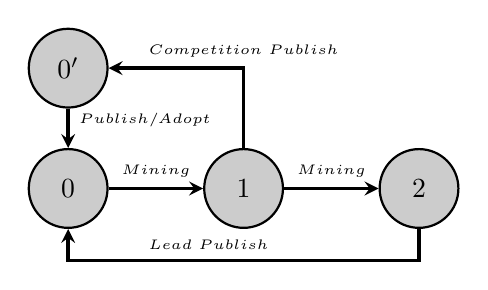
\begin{tikzpicture}
    \node[sm circ] (0) {$0$};
    \node[sm circ] (1)[right=1.2cm of 0] {$1$};
    \node[sm circ] (2)[right=1.2cm of 1] {$2$};
    \node[sm circ] (4)[above=0.5cm of 0] {$0^{\prime}$};

   	\draw [arrow] (0.east) -- node[pos= 0.5, anchor=south] {\tiny $Mining$}(1.west);
   	\draw [arrow] (1.north) |- node[pos=0.5, anchor=south] {\tiny $Competition$ $Publish$}(4.east);
   	\draw [arrow] (2.south) -- +(0,-0.4) -| node[pos=0.3, anchor=south] {\tiny $Lead$ $Publish$}(0);
   	\draw [arrow] (1.east) -- node[pos= 0.5, anchor=south] {\tiny $Mining$}(2.west);
   	\draw [arrow] (4) -- node[pos=0.3,anchor=west] {\tiny $Publish/Adopt$}(0);
   	
\end{tikzpicture}
}
\end{center}
   \caption{Abstract representation of state transtitions of eyal and sirer model for one selfish miner}
\label{fig:eyal_model}

\end{figure}
For clarification the state space and actions are modelled in Figure~\ref{fig:eyal_model}. The numbers in the states indicate the lead of the private to the public chain, where $s$ denotes the lead of the private chain compared to the public chain. We can identify a total of five different actions.
\begin{itemize}
\item $Mining$: This action means that the peer has mined a block. Mining adds the block to the private chain. It therefore causes $s$ to increase.
\item $Lead$ $Publish$: When $s$ increases to 2, the selfish miner will publish his private chain. It therefore causes $s$ to change from 2 to 0.
\item $Competition$ $Publish$: When $s$ is 1 and the selfish miner receives a block from another peer, he will publish his block of the same height from the private chain instead of the received one, to compete against the other miner. This causes a state transition to $0'$.
\item $Publish$: If the selfish miner is in state $0'$, he is in a competition situation.
The selfish miner will immediately publish his next mined block. This will cause the selfish miner to transition to state $0$.
\item $Adopt$: The selfish miner will adopt the main chain once he receives a new block in a competition situation.
\end{itemize}
Executing this protocol leads to a strict revenue increase, if the mining power is greater than $33\%$ according to \citeauthor{eyal}~\cite{eyal}.
\paragraph{Network Propagation Factor}\label{netpropfac}
\cauth{eyal} also introduced a selfish mining focused network metric, called $\gamma$. $\gamma$ is measured in competition publish situations~\ref{eyalmodel}. In a competition publish situation two competing blocks are propagated through the network. An honest peer will adopt the first block increasing his blockchain height. $\gamma$ describes the computational power fraction of the network the selfish miner block reaches before the other block. This is an advantage since now the selfish miner and the fraction he reached first start mining together on a consecutive block, securing the selfish miners block in the main chain while the competing block remains a fork.


\section{Blockchain Gossip Model}\label{gopalan}
The Blockchain Gossip Model of \citeauthor{gopalan} consists of a set of peers $P$ connected through a peer-to-peer network. Peers add blocks to the blockchain through a process called mining. 
The peer-to-peer network is modelled as an undirected Graph $H = (V,E)$.
An edge $(i,j) \in E$ represents communication possibilities between $v_i \in V$ and $v_j \in V$. 
The set of vertices is finite, such that $|V|=N \in \mathbb{N}$.
Vertices are associated with peers, such that $v_i$ represents peer $p_i \in P$.
Additionally, a directed acyclic graph $G_{p_i}(t) = (B_{G_{p_i}}(t),E_{G_{p_i}}(t))$ is associated with each peer $p_i$, at each point in time $t \in \mathbb{R+}$.
The vertex set $B_{G_{p_i}}(t) \subset \mathbb{N}$ represents the blocks known of peer $p_i$ at time $t$. The associated edge set of $E_{G_{p_i}}(t)$ represents references between blocks.
The following holds true for shorter notations:
\begin{equation}
B_G(t) = \cup_{i=1}^N B_{G_{p_i}}(t) \texttt{ and } E_G(t) = \cup_{i=1}^N E_{G_{p_i}}(t)
\label{unisondef}
\end{equation}

Furthermore, the following equations hold for the principle of blockchains:
\begin{equation}
\forall p \in P: G_{p_i}(0) = (\{0\},\emptyset)
\label{genesis}
\end{equation}
\begin{equation}
t_1 < t_2 \rightarrow B_{G_{p_i}}(t_1) \subseteq B_{G_{p_i}}(t_2)
\label{nodegrow}
\end{equation}
\begin{equation}
t_1 < t_2 \rightarrow E_{G_{p_i}}(t_1) \subseteq E_{G_{p_i}}(t_2)
\label{edgegrow}
\end{equation}

Note that in this representation $0$ denotes the genesis block described in Equation~\ref{genesis}.
$G_{p_i}(t)$ evolves over time. Blocks arrive over continuous time according to a stationary point process $A$ with intensity $\lambda$. Each block $b \in \mathbb{N}$ arrives at a random peer $p_i$.
This models peer $p_i$ mining block $b$ at time $t$ and that at this time the block is also added to $B_{G_{p_i}}(t)$.
References are added to $E_{G_{p_i}}(t)$ according to policy and depending on $G_{p_i}(t^-)$, where $t^-$ is a moment in time infinitesimally before $t$. $O_i$ denotes the set of outgoing neighbors of block $i$.

The communication is modelled as a marked point process $T_{p_i}$.
Each mark corresponds to another peer $p_j \in P\backslash \{p_i\}$.
In an epoch peer $p_i$ contacts $p_j$ and thus, adds the lowest numbered block of $B_{p_i}(t)\backslash B_{p_j}(t)$ to the set of Vertices $B_{p_j}$. If $B_{p_i}(t)\backslash B_{p_j}(t)$ is not empty, $E_{p_j}$ is also updated accordingly.

The peer-to-peer network dynamics are modelled as a continuous time rumor-spreading process with exogenous arrivals~\citep{gopalan}. Since communication is bound to the process $T_{p_i}$, the block dissemination is bandwidth limited.
Reference selection and thus $O_{p_i}$ is chosen according to longest chain policies~\citep{gopalan}.
Let $L_{p_i}(t)$ denote the set of blocks farthest away from the genesis block $0$, known to peer $p_i$ at time $t$.
\begin{equation}
L_{p_i}(t) := \{j \in B_{p_i}(t): d(j,0)\geq d(j',0), \forall j' \in B_{p_i}(t) \}
\label{policy}
\end{equation}
Let $max\_ dist(G_{p_i}(t))$ denote that distance.
Note that the set $O_{p_i} \cap L_{p_i}(t)$ is non empty. This constructs a simple directed acyclic graph. The Tree Policy~\citep{gopalan} can then be determined as $|O_{p_i}|=1$ and establishes the following relationship:
\begin{equation}
|E_{G_{p_i}}(t)| = |B_{G_{p_i}}(t)| -1
\end{equation}
Every block will have exactly one outgoing reference, according to a deterministic rule~\citep{gopalan}. \citeauthor{gopalan} assume that the block with the lower index number will be chosen.

\begin{figure}[t]
\centering
{\renewcommand{\arraystretch}{1.5}
	\begin{tabular}{|c|c|}
	\hline
	\textbf{Key Elements}		&\textbf{Short Description}\\
	\hline
	$G_{p_i}(t)$				& \footnotesize Blockchain graph representation consisting of $(B_{G_{p_i}}(t),E_{G_{p_i}}(t))$ for every peer, time variant\\
	$B_{G_{p_i}}(t)$			& \footnotesize Blockset of each peer, time variant\\
	$E_{G_{p_i}}(t))$			& \footnotesize Edgeset of each peer, time variant \\
	$T_{p_i}$					& \footnotesize The communication process for each peer, sends blocks from $p_i$ outwards\\
	$L_{p_i}(t)$				& \footnotesize The set of blocks farthest away from the genesis block\\
	\hline
	\end{tabular}
}
\caption{Overview of Key Model Elements}
\label{OverviewElements}
\end{figure}
To sum up we have given a short overview of important key elements of the model introduced by \gopalan in Table~\ref{OverviewElements}.

Bitcoin's mining protocol has the goal of fair leader election. However, deviating mining protocols show vulnerabilities in the incentive system. The above section introduced a model to analyze network properties of blockchain systems in an analytical manner. Additionally, it discussed adversarial mining protocols and the model they have been analyzed on. The next section will develop a new model, based on the Blockchain Gossip Model introduced by \gopalan. This model can then be utilized to also analyze adversarial mining strategies, such as selfish mining.











\chapter{A Network-centric Model for Selfish Mining}\label{chap:contribution}
The goal of this thesis is to analyze the relationship between selfish mining and networking effects. The model proposed by \gopalan~ appears to be suitable to analyze this relationship. It offers networking effects because it is based on rumor spreading, as well as analytical properties, such as that it can be utilized to simulate the system execution time.
The first step to analyze the relationship between selfish mining and networking effects is to identify important system factors. Based on the model introduced by \gopalan, we develop a new model, the Selfish Rumor Model, which also includes adversarial behavior. Through the combination of a rumor-spreading model and an abstract blockchain mining protocol, the impact of networking effects on selfish mining can be studied.

\section{System Factors}
Under  the  assumption  that  adversarial  mining  strategies  and  network  properties  influence each other it is important to categorize those factors and characterize their interdependencies. Factors can be split up into local and global factors, as well as network and mining properties.
\begin{figure}[t]
\centering
\small
{\renewcommand{\arraystretch}{3}
	\begin{tabular}{|c|c|c|c|}
	\hline
	&\textbf{Local Factors}		&\textbf{Global Factors}		&\textbf{Adversarial Factors}\\
	\hline
	\textbf{Network Factors}		&\footnotesize \makecell{Network Graph Topology \\ Network Size \\ Bandwidth Distribution \\} 		&\footnotesize \makecell{Geographic Location \\ Topological Location \\ Bandwidth \\} 
	&\footnotesize \multirow{2}{*}{\makecell{Number of Selfish Miners \\ Mining Power of Selfish Miners}}\\
	\cline{1-3}
	\textbf{Mining Factors}			&\footnotesize \makecell{ Mining Power Distribution \\ Difficulty}		&\footnotesize \makecell{Mining Power \\ Mining Strategy} &\\
	\hline
	\end{tabular}
}
\caption{Key factors influencing the selfish rumor model}
\label{keyfactors}
\end{figure}
\subsection{Network Factors}
A blockchain system is a distributed system and utilizes a network to propagate information. As such the network behavior is important for the blockchain system. Network factors influence how information is spread. Those factors are visualized in Table~\ref{keyfactors}. An important characteristic is how fast information is spread. On a global level this is highly influenced by how big the network is. In addition to network size, the network graph topology also plays a major role in how information is propagated through the network. In general a more densely connected network can propagate information faster to each peer. Another crucial factor is bandwidth distribution. The Bandwidth of a peer determines at what rate he can communicate. On a given network size the combination of bandwidth distribution and network graph topology influences drastically how fast information can spread. As an example let us consider an exponential degree distribution and an exponential bandwidth distribution. On the one hand information will spread reasonably fast, when a high bandwidth node also has a high degree. On the other hand if a node with a very low bandwidth has a high degree, he will become a bottleneck.

From a local point of view the location of a peer becomes important. Both geographic and topological location determine how fast a peer receives and sends information. Together with the amount of bandwidth the location also determines how much information is routed through that specific peer. Generally speaking a more central peer receives and sends information faster and also becomes a intermediate routing point more often. One can measure the centrality of a node by analyzing his betweenness centrality. The betweenness centrality is a measure on how many shortest paths a node lies between any other pair of two nodes. 
\subsection{Mining Factors}
Additionally, in a blockchain system key factors include mining factors. Those factors influence the mining process of each individual miner. On a global scale mining power distribution and difficulty are characteristic. Difficulty determines at which rate a new block is introduced to the network. Mining power distribution determines, where the new block is how likely to arrive. They are both key factors influencing the average block propagation, since an ill combination of both can lead to network congestion. As an example consider a peer with a high relative mining power, who only has one outgoing connection to the network. This one connection is clearly a bottleneck prone to lead to congestion. With a low difficulty the peer will mine many blocks in a short amount of time and will flood the peer connecting him to the network. This will result in an overall higher average block propagation time.

From a local point of view a miners mining process is mainly influenced by his mining power and the executed mining strategy. If a miner recruits additional computing power, he will gain increased mining power and produce more blocks. If a miner executes an adversarial mining strategy such as selfish mining in contrast to honest mining, he will have a different reference selection and a different block publishing behavior.

\subsection{Adversarial Factors}
Adversarial factors also influence a blockchain system. Because of the mining protocol a blockchain system faces additional threads outside of adversaries attacking the underlying network structure. Peers can execute block withholding strategies such as selfish mining. By executing selfish mining strategies the forkrate of the blockchain is increased and the overall growth decreased. Multiple selfish miners escalate this problem. Multiple selfish miners work against each other, but the power threshold above which a selfish miner gains revenue decreases proportionally to the number of selfish miners\ref{multi_sm}.


We can denote that the network, mining and adversarial factors mentioned above play a crucial part for the behavior of the overall system. It is therefore important to select those factors carefully and construct scenarios which analyze a wide variety of possible system factor combinations. In the next section we will now introduce the Selfish Rumor Model.

\section{Selfish Rumor Model}\label{selfishmodel}
The selfish miner behaves different to an honest miner and therefore can be modeled by altering the reference selection and communication process. The reference selection process is policy driven, and can thus be modified by providing a new selfish policy. However, for the analysis of \gopalan~ the edge set is only represented in an abstract form, since at most the height of a block is important. As a result, specifics concerning the edge set are never discussed. For selfish mining to be implemented into the model, the reference selection process becomes very important and has to be further specified.
\paragraph{Reference Selection Process Specification}
\gopalan~ introduce an edge set $E_{G_{p_i}}(t)$ for each peer for each point in time. Those edges represent selected references.
Additionally, we will introduce the notion of a Topblock $b_{{top}_{pi}}$.
The following rules apply:
\begin{enumerate}
\item $b_{{top}_{pi}}(t) \in L_{p_i}(t)$
\item If peer $p_j$ updates peer $p_i$ with a block $b'$ at time $t$, $b_{{top}_{pi}}(t) = b'$ if the height of $b'$ is strictly greater than the height of the previous Topblock $b_{{top}_{pi}}(t^-)$.
\item If on an event of $A$ a new block $b$ arrives to peer $p_i$ at time $t$, he will select $b_{{top}_{pi}}(t^-)$ as the parent reference of $b$. As a result $(b,b_{{top}_{pi}}(t^-)$ will be added to $E_{G_{p_i}}(t))$ and will be communicated through the network. Furthermore, $b_{{top}_{pi}}(t)$ will be set to $b$, such that $b_{{top}_{pi}}(t) = b$.
\end{enumerate} 
Through the above described rules reference selection is deterministically defined. It binds reference selection to the block arriving first to a peer. This is important, since a clear reference selection definition is crucial for estimating the success of selfish mining. The remainder of the section will discuss the new Selfish Rumor Model.

\paragraph{Selfish Rumor Model}
The Selfish Rumor Model is based on the Blockchain Gossip Model introduced by \gopalan . The construction of the Selfish Rumor Model can be seen as a modification of the Blockchain Gossip Model and is best explained in that manner. However, introducing adversarial mining strategies and altering key factors such as mining power distribution, changes the new model in such a drastic way that it has to be considered a new model.

The first aspect to be modified is the communication process. 
Key idea of selfish mining is block withholding. The selfish miner possesses three blockchain representations. 
\begin{itemize}
\item $G_{SM_{public}}(t)$: which is updated by other peers.
\item $G_{SM_{comm}}(t)$: which is used to update other peers.
\item $G_{SM_{private}}(t)$: with the following relations:
		\begin{itemize}
		\item $G_{SM_{public}}(t)\subseteq G_{SM_{private}}(t)$.
		\item $G_{SM_{private}}(t)\backslash G_{SM_{public}}(t)$ represents blocks mined but unpublished by the selfish miner.
\end{itemize}		
\end{itemize}


\begin{figure}[t]
\begin{center}
\resizebox{\columnwidth}{!}{%
  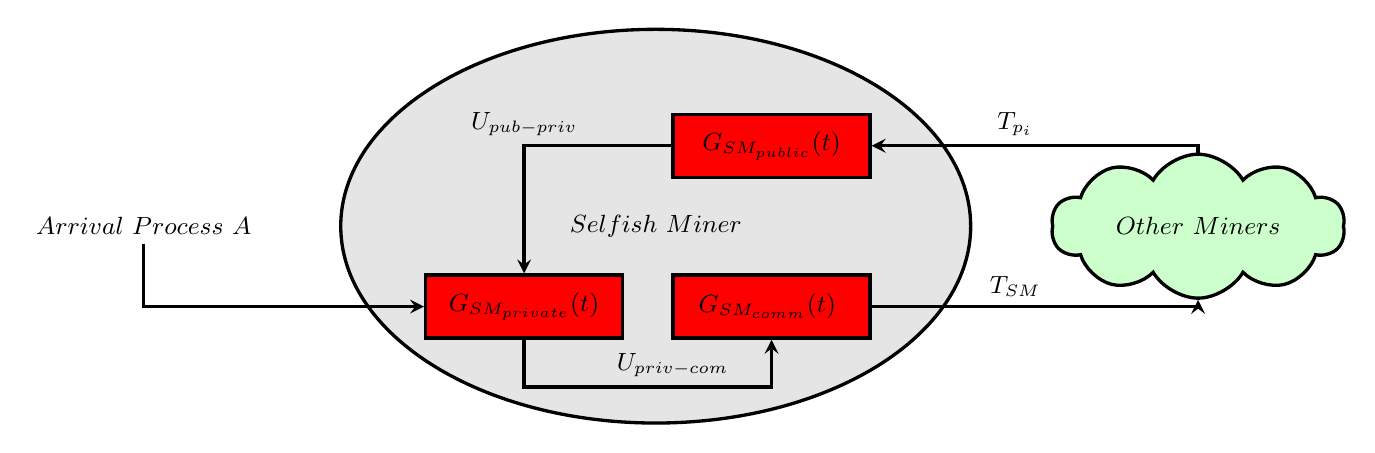
\begin{tikzpicture}
  \small
    \node[sm node] (1) {$Selfish~Miner$};
    \node(2) [left = 1cm of 1] {$Arrival~Process~A$};
    
    \node[block] (3) [above right = 0.6cm and 0.2cm]{$G_{SM_{public}}(t)$};
    \node[block] (5) [ below =1.2cm of 3 ]{ $G_{SM_{comm}}(t)$ };
	\node[block] (4) [left=0.6cm of 5]{$G_{SM_{private}}(t)$};    
    
    \node [cloud,fill=green!20, draw,very thick,cloud puffs=10,cloud puff arc=120, aspect=3, inner ysep=1em, right=1cm of 1](6) {$Other~Miners$};
    
   	
   	\draw [arrow] (2) |- (4);
   	\draw [arrow] (3) -| node[anchor=south] {$U_{pub-priv}$}(4);
   	\draw [arrow] (4.south) -- +(0,-0.6) -| node[pos=0.3, anchor=south] {$U_{priv-com}$}(5);
   	\draw [arrow] (6) |- node[pos=0.78,anchor=south] {$T_{p_i}$}(3);
	\draw [arrow] (5) -| node[pos=0.22,anchor=south] {$T_{SM}$}(6);    
\end{tikzpicture}
}
\end{center}
   \caption{Abstract representation of model entities and communication processes}
\label{fig:model_vis}

\end{figure}
The concept has been visualized in Figure~\ref{fig:model_vis}.
A total number of five processes is used to let all entities interact with each other.
\begin{itemize}
\item $Arrival~Process~A$: Blocks arrive to the selfish miner over the external arrival process $A$.

\item $T_{p_i}$: Ensures blocks from other peers are communicated to $G_{SM_{public}}(t)$.
\item $U_{pub-priv}$: Ensures that $G_{SM_{public}}(t)\subseteq G_{SM_{private}}(t)$ holds true, meaning $U_{pub-priv}$ updates $G_{SM_{private}}(t)$, when new blocks arrive to $G_{SM_{public}}(t)$ from other peers.
\item $U_{priv-com}$: Updates $G_{SM_{comm}}(t)$ according to $G_{SM_{private}}(t)$ and the selfish mining rules $S$.

\item $T_{SM}$: Ensures other peers are updated with blocks from $G_{SM_{comm}}(t)$.
\end{itemize}

Peer $SM \in P$ has an associated policy slightly different to the policy described in the Gopalan model~\ref{policy}. Note that to follow the Tree Policy~\citep{gopalan}, a deterministic rule has to be established for the case that $|O_{SM} \cap L_{SM}(t)| > 1$.
Assume that $SM$ has the knowledge of the set of blocks mined through him, $M_{SM}(t) \subset B_{G_{SM}}(t)$. $SM$ will set 
\begin{equation}
(L_{SM}(t) \cap M_{SM}(t)) \neq \emptyset \rightarrow L'_{SM}(t) \subset ( L_{SM}(t) \cap M_{SM}(t)) 
\label{smpolicy}
\end{equation}
It then follows that $|L'_{SM}(t)|=1$.
This modified tree policy sets references according to the original selfish mining protocol described by \citeauthor{eyal}.

$S$ is a set of rules which describes how $G_{SM_{private}}(t)$ updates $G_{SM_{comm}}(t)$. The rules have to follow the state description of \citeauthor{eyal}~\ref{eyalmodel}. Therefore we need a state variable describing the difference between private and public chain.
Let $s$ be the state variable determining selfish mining actions~\citep{eyal}.
Then $s$ can be described as a difference between $G_{SM_{private}}(t)$ and $G_{SM_{public}}(t)$.

\begin{equation}
max\_ dist\_mined(G_{SM_{private}}(t)) := d(j,0), j \in M_{p_i}(t)
\end{equation}
\begin{equation}
s(t) := max\_ dist\_mined(G_{SM_{private}}(t)) - max\_ dist(G_{SM_{public}}(t))
\end{equation}

Let $t_{inc}$ refer to the set of times, where $s$ increased and analogous $t_{dec}$ refer to the set of times, where $s$ decreased.
Selfish mining is protocol, which needs a formulation of states in order to be characterized. \citeauthor{gopalan} introduced $t^-$ as a point in time infinitesimally before $t$. In addition to describe selfish mining a function is needed to access the point in time where $s$ changed last.
Let $f_{-1}(t)$ be a function that outputs the point in time, where $s$ changed the latest before $t$.
Now all tools are available to characterize the selfish mining protocol on top of the stochastic network model introduced by \citeauthor{gopalan}.

$U_{priv-com}$ can be characterized through four kind of update actions. Analogous to Subsection~\ref{eyalmodel}, those actions are $Lead~Publish$, $Competition~Publish$, $Publish$ and $Adopt$. $Mining$, the fifth action described in Subsection~\ref{eyalmodel}, is modelled through the arrival process.
This can be used to model the selfish mining protocol desribed by \citeauthor{eyal}.
\begin{enumerate}
\item $Lead~Publish$: Assume $t \in t_{inc}$ and $s(t) \geq 2$, then $U_{priv-com}$ updates $G_{SM_{comm}}(t)$, such that $G_{SM_{comm}}(t) = G_{SM_{private}}(t)$. Once the selfish miner has established a lead of two blocks against the public chain, he will update the blockchain representation used for communication towards other peers. In other words, he publishes the private chain.
\item $Competition~Publish$: Assume $t \in t_{dec}$, $s(t) = 0$, $s(f_{-1}(t)) = 1$, $s(f_{-1}(t)^-) = 0$. This means that the selfish miner mined a block, did not publish it and now received a block from another of the same height. This leads to the competition scenario. Accordingly, $U_{priv-com}$ updates $G_{SM_{comm}}(t)$, such that it includes the subgraph induced by the nodes on the paths between $L'_{SM}(t)$ and ${0}$. The selfish miner will publish the block, which caused the private chain to lead by one against the public chain, before he received a new block. This transitions to 
\begin{equation}
0'(t) \rightarrow \left( t \in t_{dec} \wedge s(t) = 0 \wedge s(f_{-1}(t)) = 1 \wedge s(f_{-1}(t)^-) = 0\right)
\end{equation}
This situation $0'$ is also shown and visualized in Subsection~\ref{eyalmodel} and causes the selfish miner to execute honest mining for only the next step. \label{comppub}
\item $Publish$: Assume $0'(t^-)=\top$ and $t \in t_{inc}$, $U_{priv-com}$ updates $G_{SM_{comm}}(t)$, such that it includes the subgraph induced by the nodes on the paths between $L'_{SM}(t)$ and ${0}$. The selfish miner will publish his newly mined block, because he was previously in $0'$.
\item $Adopt$: Assume $0'(t^-)=\top$ and $s(t)=-1$, then $U_{priv-com}$ updates $G_{SM_{comm}}(t)$, such that $G_{SM_{comm}}(t) = G_{SM_{private}}(t)$. The selfish miner will adopt the public chain, because he was previously in $0'$.
\end{enumerate}
The above section introduced a new model, the Selfish Rumor Model.
However, a number of core contributions of \gopalan still hold true, such as the results proofing that Poisson processes are a good approximation of the real process. Furthermore, since peer-to-peer networks based on regular grids, regular trees and random geometric networks are already proven to be non scaleable the Selfish Rumor Model can rely on regular-random networks. The Selfish Rumor Model utilizes the tree-policy. \gopalan stated that any blockchain constructed under the tree policy is one-ended as long as the network is stable. A blockchain is one-ended if there are infinitely many confirmed blocks and a stable network means an infinite sequence of times, where the system is consistent. Since selfish mining does not influence the system to produce an infinite amount of inconsistent system times, the network has to considered stable. As a result the proof on the one-endedness of the blockchain DAG also holds true.

Through the combination of rumor-spreading mechanisms for an abstract network layer representation and adversarial mining strategies, this model can be used to analyze the relationship between the selfish mining attack and networking effects.





\chapter{Evaluation}\label{chap:evaluation}
The following section utilizes the simulative implementation of the Blockchain Gossip Model to evaluate the relationship between selfish mining and networking effects. Additionally, the model will be validated against data provided by~\cauth{gopalan}~and real world data of the Bitcoin system.
\section{Simpy Blockchain Simulator}
The core implementation is based on simpy~\cite{simpy}. Simpy is a discrete event simulator written in python. As a result the Simpy Blockchain Simulator is also written in python. 
The Selfish Rumor Model consists mainly of four parts. 
\begin{itemize}
\item Networkgraph representation
\item Blockchain representation
\item Block Arrival Process representation
\item Communication Process representation
\end{itemize}
The network graph is represented by an adjacency matrix. The blockchain representation is a set of blocks and a set of edges for each peer, which are developing over time. The block arrival process and the communication process are modeled as a Poisson process~\cite{poisson}. This is mirrored in a Simpy process with an exponentially distributed interarrival time between scheduled events.
On each event of the block arrival process a block arrives at a random peer. This means that the event triggered by the block arrival process updates the blockchain datastructure accordingly.
At each event of the communication process $T_i$ a peer $p_i$ tries to update a certain peer $p_j$ according to the epoch associated with the event. This results in a comparison between the datastructures associated with $p_i$ and $p_j$ and an update of $p_j$, if it is possible.

Even though the basic implementation is simple, there are various parameters which influence the system behavior greatly. The following list shall give an overview:
\begin{itemize}
\item Average of interarrival times - This is the rate of block arrival process and communication process trigger events. 
\item Topology of the network graph - The network resulting from the adjacency matrix has a great influence on the behavior of the system.
\item Block selection - In a scenario, where multiple blocks could be transferred from one peer to another, one block has to be selected. How this block is selected influences system baviour.
\item Network size - This is the number of peers.
\item Mining power distribution - The mining power distribution influences the peer selection. Peer selection is the process of deciding which peer gets the new block once the block arrival process triggers an event.
\end{itemize}
The above discussed parameters can be modified in order to capture different systems.

\section{Validation of the Simpy Blockchain Simulator}
In the following section the Simpy Blockchain Simulator is validated against synthetic experiments published by the original authors of the blockchain gossip model. Additionally real world data from Bitcoin will be additionally used to validate the legitimacy of the Simpy Blockchain Simulator. This will lay the foundation for further analysis concerning the network and selfish mining. 
\subsection{Validation of Simulator against~\cauth{gopalan}}\label{gopalananalysis}
In the synthetic data experiments of~\cauth{gopalan}~they analyze the the network for 10, 20 and 30 peers. The network topology is a complete graph. Thus, the adjacency matrix is the unit matrix. 
The authors introduce four key metrics to analyze the system. Time to Consistency as the average time an inconsistent system needs to reach a state of consistency. Cycle Length as the sum of the average time to consistency and the average of the time the system stays consistent. Consistency Fraction as the average fraction of peers that are consistent at each point in time. Age of Information as the average number of blocks an average peer is away from the consistency state. \\
All metrics mentioned above refer to the term consistency. The Consistency is defined as $B_G(t)$~\ref{unisondef}, the unison of all blocks produced by the block arrival process $A$.
In order to evaluate to capture the same system, that was analyzed by the authors, the parameters are setup similar.
These metrics can be used to verify whether the Simpy Blockchain Simulator is achieving similar numbers to the implementation of~\cauth{gopalan}. As for the parameter setup the interarrival time of the communication process is set to $1s$. The interarrival time of the block arrival process is a variable. The network topology is a complete graph. In a scenario, where multiple blocks could be transferred from one peer to another the block with the lowest index number is chosen. The network size is set to 10, 20 and 30 peers accordingly. The mining power distribution is uniform.
\begin{figure}[tbp]
	\begin{subfigure}[b]{0.5\textwidth}
		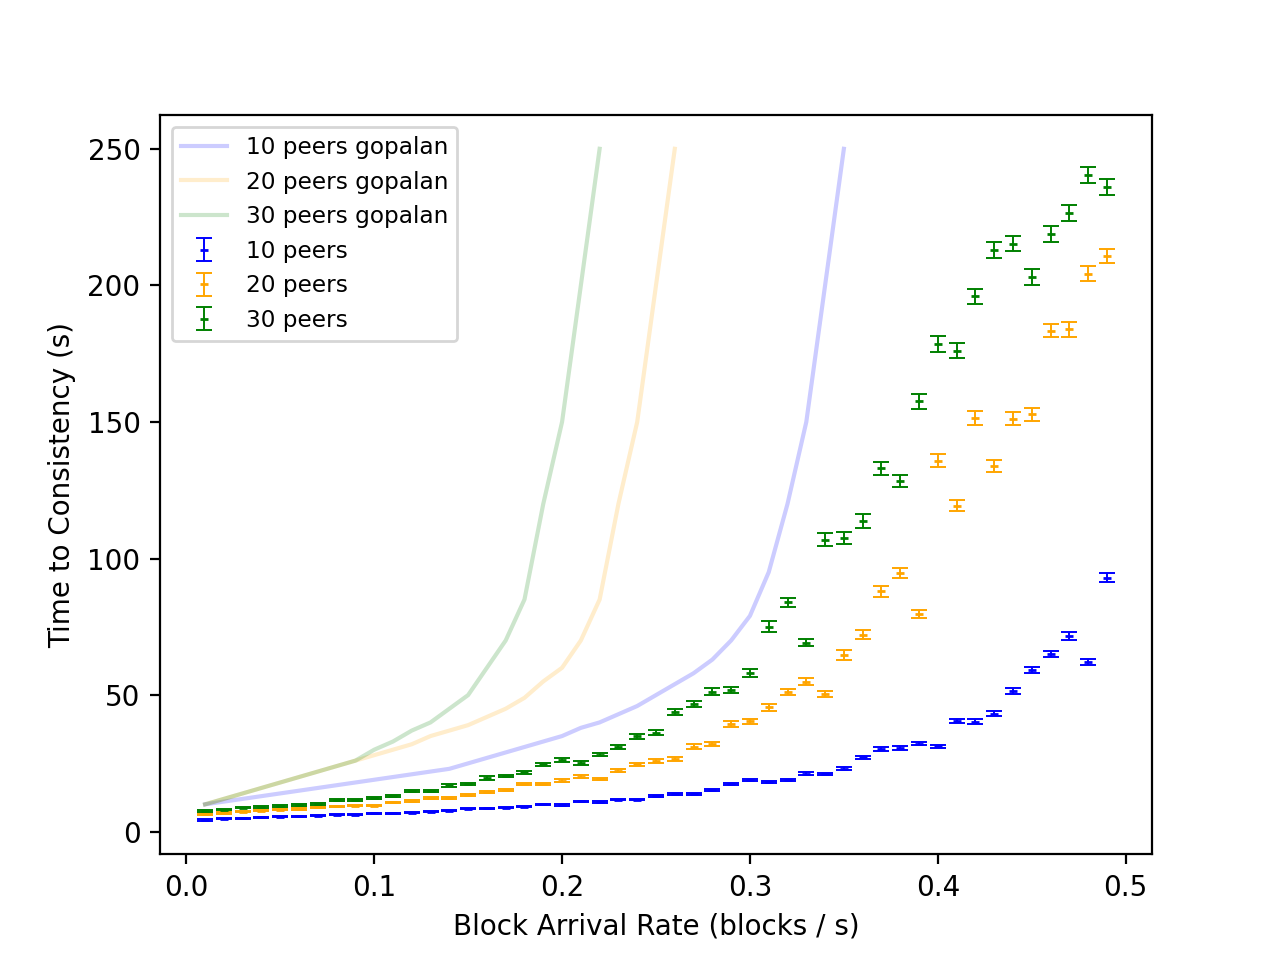
\includegraphics[width=\textwidth]{figures/gopalan_figures/time_to_consistency.png}
		\caption{ Time to Consistency}
		\label{fig:gopalan_ttc}
	\end{subfigure}
	\hfill
	\begin{subfigure}[b]{0.5\textwidth}
		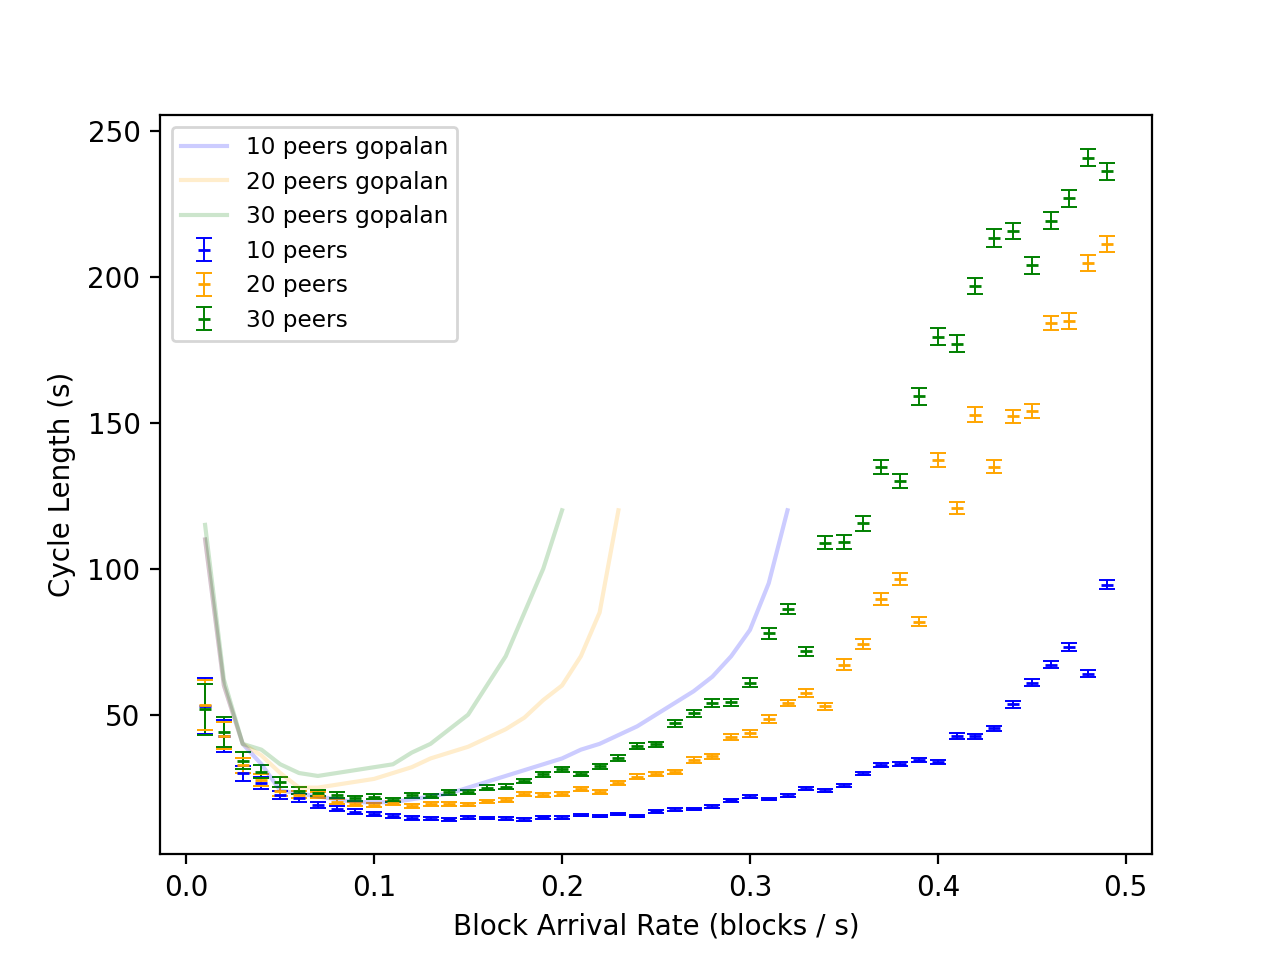
\includegraphics[width=\textwidth]{figures/gopalan_figures/cycle_length_avg.png}
		\caption{ Cycle Length}
		\label{fig:gopalan_cl}
	\end{subfigure}
	\hfill
	\begin{subfigure}[b]{0.5\textwidth}
		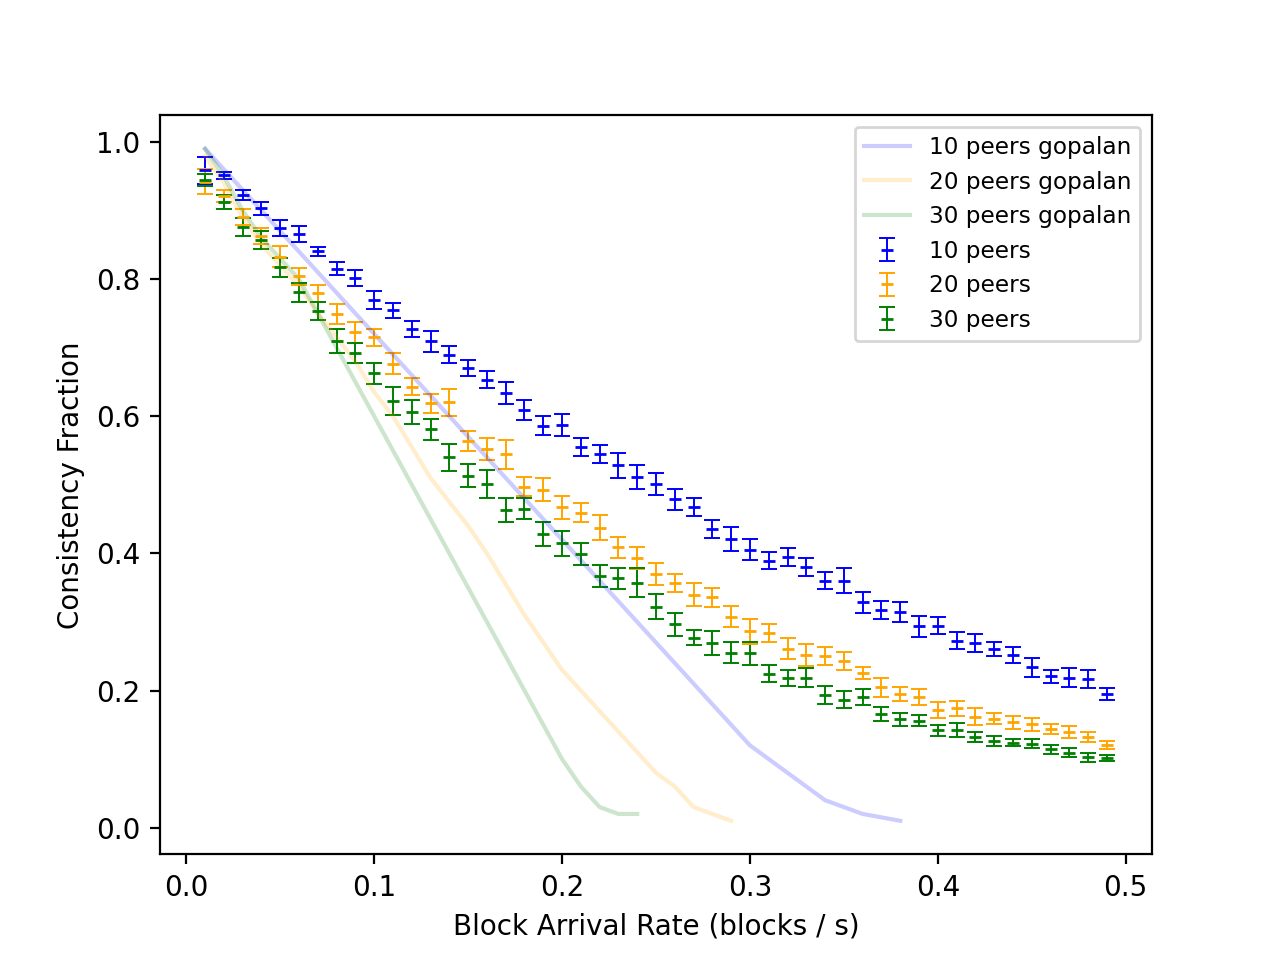
\includegraphics[width=\textwidth]{figures/gopalan_figures/consistency_fraction.png}
		\caption{ Consistency Fraction}
		\label{fig:gopalan_cf}
	\end{subfigure}
	\hfill
	\begin{subfigure}[b]{0.5\textwidth}
		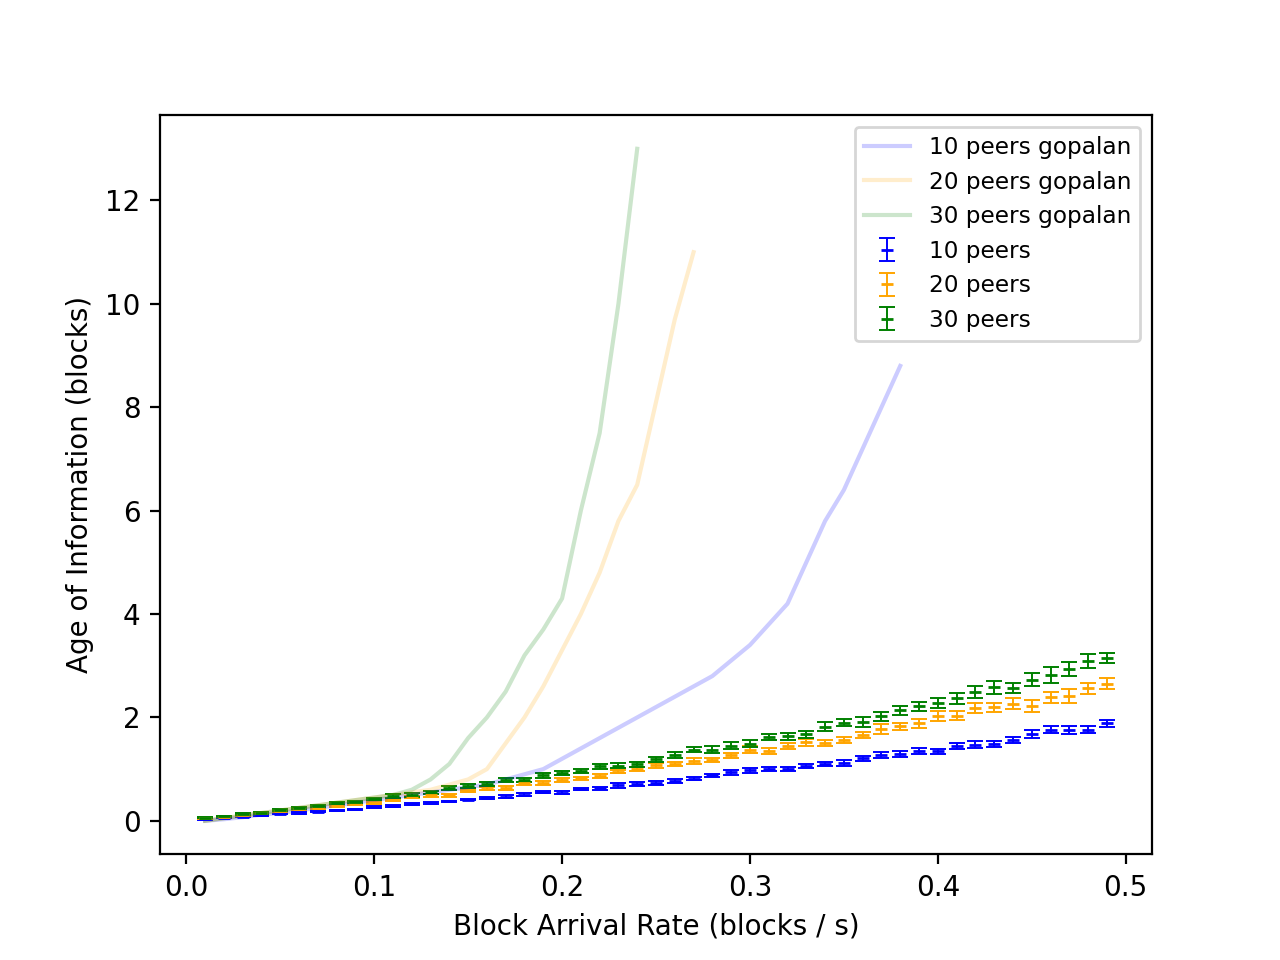
\includegraphics[width=\textwidth]{figures/gopalan_figures/age_of_information.png}
		\caption{ Age of Information}
		\label{fig:gopalan_aof}
	\end{subfigure}
	\caption{Comparison between Simpy Blockchain Simulator and values produced by~\cauth{gopalan}}
\end{figure} 
The metrics of time to consistency and cycle length are very closely related, because both rely on the time the system needs to reach consistency.
Figure~\ref{fig:gopalan_ttc} and Figure~\ref{fig:gopalan_cl} show this close relationship. Additionally the comparison between the Simpy Blockchain Simulator shows a very similar tendency in both metrics. Especially in Figure~\ref{fig:gopalan_ttc} it is observable that the curve has the same shape, only flatter. Figure~\ref{fig:gopalan_ttc} shows that peernumber and block arrival rate are proportional to the average time to consistency. Since cycle length is the sum of the average time to consistency and the average of the time the system stays consistent the same behavior can be observed in Figure~\ref{fig:gopalan_cl}. Additionally Figure~\ref{fig:gopalan_cl} shows that for very small numbers for the block arrival rate the cycle length increases again. When the system has a low block arrival rate the system tends to stay longer in a state of consistency, which is due to the fact that the idle time increases.\\
Consistency fraction and age of information are both metrics measuring the consistency of an average peer. The consistency fraction is the fraction of peers, which have a blockset equal to $B_G(t)$~\ref{unisondef}. For both the simulation results by~\cauth{gopalan}~and the Simpy Blockchain Simulator we can observe, that the consistency fraction decreases with an increasing blockrate and peer number. While the exact numbers do differ, similar shapes can again be observed.\\
The age of information metric analyzes how much an average peer differs from $B_G(t)$~\ref{unisondef}. It showcases an increase for an increasing blockrate and peer number.
The differences indicate that information spreads faster in the Simpy Blockchain Simulator. After a brief discussion with~\cauth{gopalan}, they confirmed that this might be due to the fact, that in the simpy version communication processes are handled truly concurrently.	

\subsection{Validation of Simulator against Bitcoin data}
This section validates the model against a real world blockchain system, the Bitcoin network. The Selfish Rumor Model implements an abstract network model of blockchain systems, simulating block creation and block propagation.
\cauth{neudecker-atc16} monitor the Bitcoin network and obtain data of, for example, the current block propagation delay distribution~\cite{BitcoinNetworkMonitor}. Since the model can be used to analyze blocks and their propagation, the current block propagation delay distribution is a suitable metric to compare the Selfish Rumor Model against the real world system.\\
Bitcoin block propagation has two distinct characteristics. The distribution has a high peak at around $~400ms$ and a significant long tail, with block delays going up to $30s$. Since the whole dataset contains many outliers, $5\% $ of the largest delays are filtered out. This data is then used to match parameter setups of the Selfish Rumor Model against Bitcoin and find setups offering a similar block propagation.\\
To achieve a similar block propagation one can mainly analyze the topology of the network graph and the communication process rate.
The current Bitcoin network has an unknown topology. The original protocol described an algorithm, where a peer tries to maintain at least 8 connections~\cite{tschorsch}. This would result in a random regular graph as network topology. However, analysis of the Bitcoin network comes to a different conclusion.\\
For example \cauth{baumann2014exploring} found strong indicators for a scale-free degree distribution.
Additionally, the FIBRE network and Compact Blocks were introduced to enable faster block propagation~\cite{measurement}. This results in a network topology, which cannot be captured by single graph representation.\\
Since the Selfish Rumor Model uses one single graph representation the objective is to utilize a topology and minimize the Root-Mean-Square-Error(RMSE). The RMSE is the standard deviation of the prediction errors~\cite{RMSE}. Since the Selfish Rumor Model Simulator can predict block propagation of Bitcoin, we can measure the error compared to Bitcoins block propagation utilizing the RMSE. Therefore, either a regular random graph or a scale free graph should be chosen as a network topology for the Selfish Rumor Model. 
\begin{figure}[tbp]
	 \begin{subfigure}[b]{0.48\textwidth}
		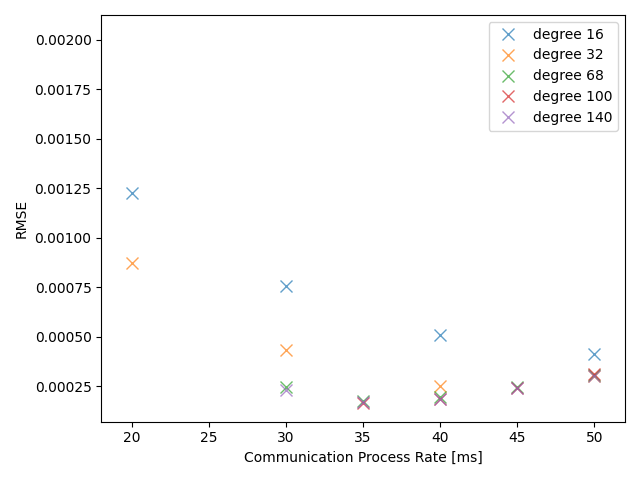
\includegraphics[width=\textwidth]{figures/RMSE_95.png}
		\caption{RMSE between Selfish Rumor Model regular-random Graph and Bitcoin}
		\label{fig:RMSE}
	\end{subfigure}
	\hfill
	\begin{subfigure}[b]{0.48\textwidth}
		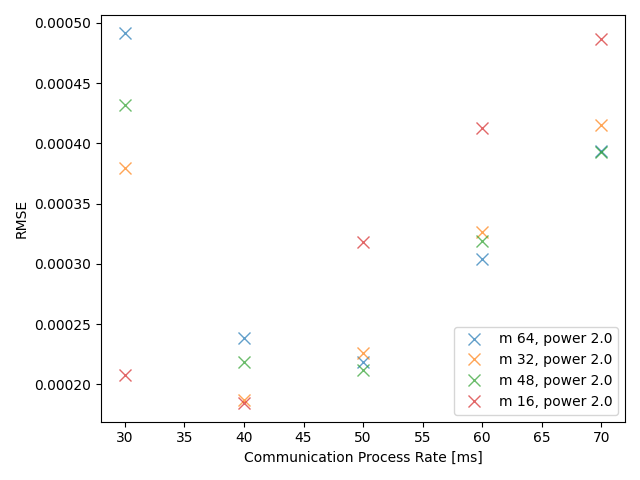
\includegraphics[width=\textwidth]{figures/RMSE_95_barabasi.png}
		\caption{RMSE between Selfish Rumor Model scale-free Graph and Bitcoin}
		\label{fig:RMSEBar}
	\end{subfigure}
	\hfill
	\begin{subfigure}[b]{0.48\textwidth}
		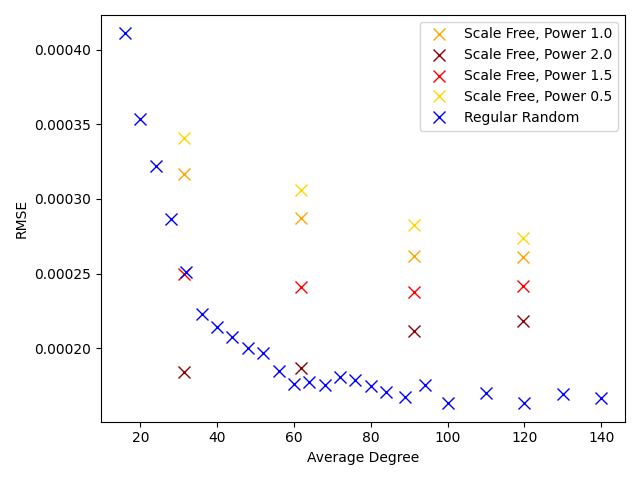
\includegraphics[width=\textwidth]{figures/rmse_min.png}
		\caption{Minimum RMSE value in random-regular graph and scale-free graph}
		\label{fig:minRMSE}
	\end{subfigure}
	\hfill
	\begin{subfigure}[b]{0.48\textwidth}
		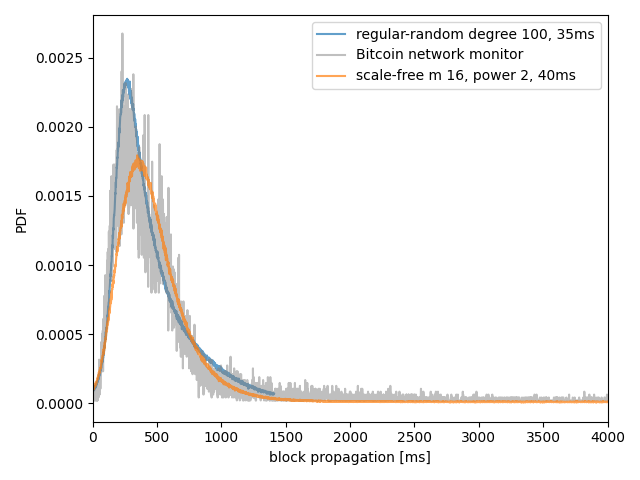
\includegraphics[width=\textwidth]{figures/propagation_histogram_withBitcoin.png}
		\caption{Selfish Rumor Model Model Block Propagation Distribution and Bitcoin}
		\label{fig:SRMBitcoin2}
	\end{subfigure}
\caption{Selfish Rumor Model Experiments in comparison with Bitcoin, 500 Peers}
\label{fig:SMRBitcoin}
\end{figure}
Figure~\ref{fig:SMRBitcoin} shows the most important results of various experiments carried out to minimize the RMSE between the simulations and Bitcoin. It also offers a comparison between the scale-free topology shown as orange and the regular random topology shown as blue. Since both topologies differ only in the degree distribution, we can compare both by their average degree respectively. All block delays were grouped in $1ms$ steps. All setups were repeated 100 times to ensure statistical significance.\\
Figure~\ref{fig:RMSE} shows the RMSE for 16, 32, 68, 100, 140 degrees and various communication process rates in comparison to Bitcoin. The lowest RMSE, $0.00016$, was achieved by 100-regular-random graph with a communication process rate of $35ms$. This parameter setup is referred to as $RegRan$.\\
In Addition the results for a 16- and 32-regular-random graph are also shown in Figure~\ref{fig:RMSE}. A 32 degree regular random graph is used by~\cauth{gopalan}~to evaluate against Bitcoin data. However, the RMSE-values are significantly higher than those of the 100-regular-random graph. This is most likely due to the usage of the FIBRE relay network and Compact Blocks in Bitcoin, which decreases block propagation delay. Additionally, all curves have a clear tendency towards a specific communication rate minimizing the RMSE.\\
This is also the case for scale-free networks, as is visualized in Figure~\ref{fig:RMSEBar}. For each topology there is one minimum communication rate, minimizing the RMSE against Bitcoin block propagation delay distribution. The scale-free network is generated over the Barabasi-Albert model~\cite{BarabasiAlbert}. This algorithm has three determining parameters. The number of vertices, $m$ for the number of edges generated for each vertex and a power factor. Since the lowest RMSE was always achieved for the power factor $2$ Figure~\ref{fig:RMSEBar} shows only the RMSE for power $2$.\\
The lowest achieved RMSE, $0.00018$, for scale free networks was for an average of 16 m, a power factor of 2 and a communication process rate of 40ms. This parameter setup is referred to as $ScaFre$.\\
Both topologies achieve quite low RMSE values. However, Figure~\ref{fig:minRMSE} visualizes the difference between the minimum RMSE values achieved for each average degree for both random regular and scale free graphs.
Regular random graphs lower the RMSE values for an increasing average degree, until an average degree of 80. Above an average degree of 80 the RMSE values remain quite constant.\\
The analyzation of parameter setups for scale free networks is more complex. Scale-free networks, in terms of the Barabasi-Albert model, have the parameter m, which can be used to control the average degree of the network. Additionally scale-free networks have a power factor, which controls the preferential attachment process. Since 4 different power factors were analyzed for each setup, Figure~\ref{fig:minRMSE} visualizes 4 datapoints above each other for each average degree. We can observe that for $m=16$ and for $m=32$ the achieved RMSE values are the lowest for power factor 2 and a communication process rate of 40ms.\\
Figure~\ref{fig:SRMBitcoin2} visualizes the block propagation distribution from the Selfish Rumor Model for both tested topologies in their minimum configuration and Bitcoin. The regular random graph models the peak closer. The scale free network cannot model the peak as good as the regular random network, but the curve shows more distinctly the longtail behavior. The better model for lower delays achieves a better RMSE value, since lower delays contain much more data points. Since data points above 1500ms are rare for Bitcoin, the exact modelling of the long tail does not impact the RMSE value as much. Nonetheless, both parameter setups are valuable to establish a validated Selfish Rumor Model Setup.\\
We conclude this section by establishing two parameter setups. The minimum configuration for regular random networks is called $RegRan$ and the minimum configuration for scale-free networks is called $ScaFre$. Both are discussed in their differences in the above chapter exhaustively. However, there are also characteristics both share.\\
The interarrival time of the block arrival process is set to 600s. In a scenario, where multiple blocks could be transferred from one peer to another the block with the earliest arrival time is chosen. The number of peers is set to 500 and the mining power distribution is exponential. Additionally Simulations are always carried out 100 times to ensure statistical significance.
Those parameter setups, $RegRan$ and $ScaFre$ are used for following evaluations.

\section{Selfish Mining and Networking Effects}
Networking effects and selfish mining can be analyzed from a global and a local point of view, cf. Table~\ref{keyfactors}. The system analysis introduced by~\cauth{gopalan}~assesses the system mainly in terms of consistency and blockchain growth, as discussed in the previous section. Both, blockchain growth and consistency, are influenced by adversarial mining strategies such as selfish mining. Additionally, selfish mining is influenced by networking factors.

\subsection{Selfish Mining in homogeneous Network Setting}
\citeauthor{eyal}~\cite{eyal} discovered a relationship between the relative computational power and the resulting $revenue~gain$. They described that an increase in networking propagation factor and relative computational power results in an increased $revenue~gain$. Additionally to the metrics of $revenue~gain$ and network propagation factor $\gamma_{hr}$ we introduce two other metrics. Those are $growth$ and $fork~rate$. $growth$ describes the length of the blockchain relative to the number of produced blocks and $fork~rate$ describes the number of forks relative to the number of blocks~\cite{BlockPropOld}. A high $growth$ means that most produced blocks end up in the longest chain. If the $fork~rate$ is significantly smaller than $1-growth$ this implies that forks tend to contain many blocks. If it is close to equal forks are mostly consisting of one block.\\
In a homogeneous network every peer has the same degree and the same bandwidth. Such a network setup is the $RegRan$ setup and it can be used to analyze selfish mining in a scenario without any networking advantage.
\begin{figure}[tbp]
	 \begin{subfigure}[b]{0.5\textwidth}
		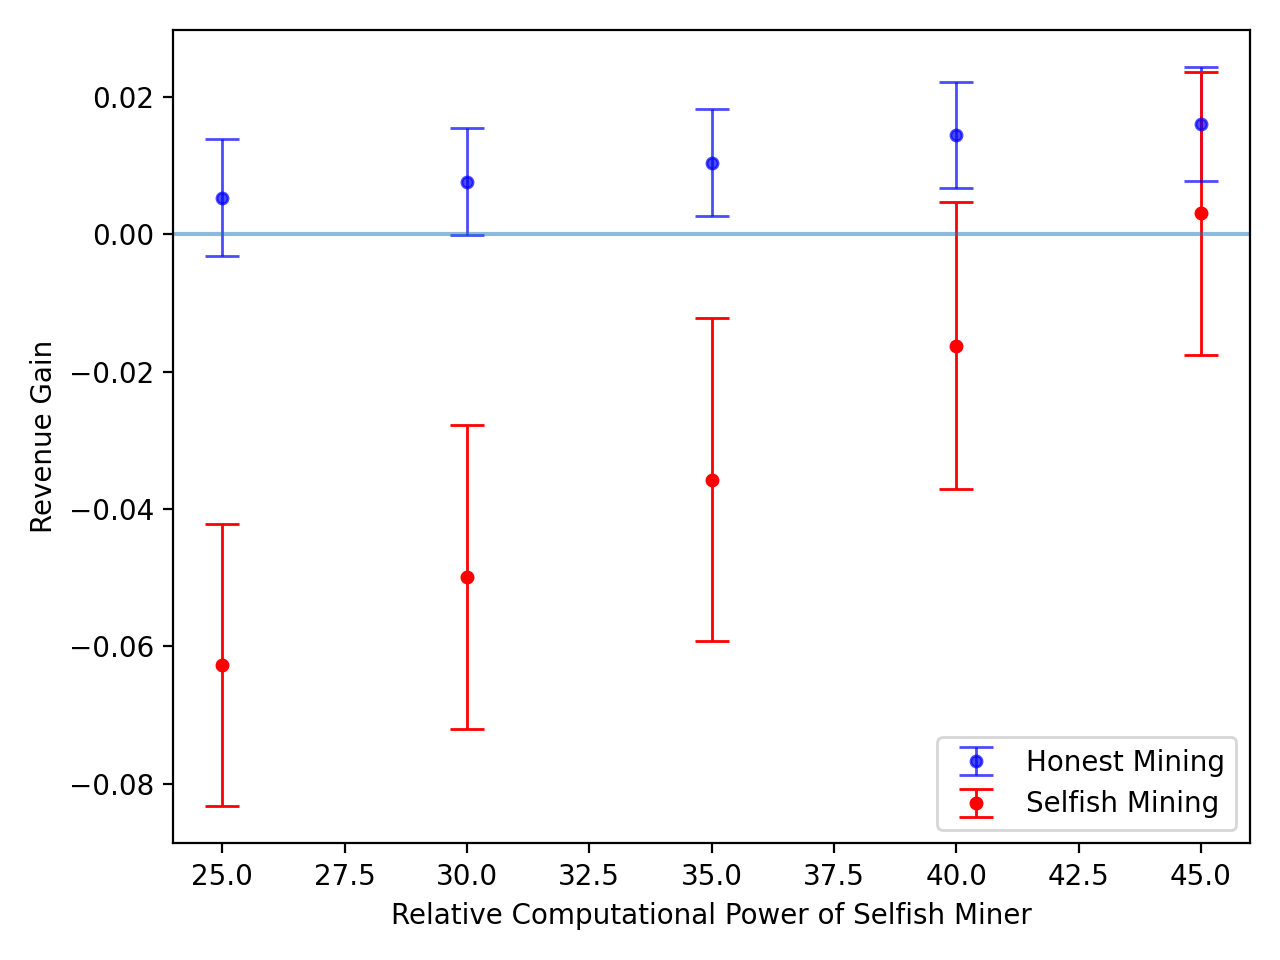
\includegraphics[width=\textwidth]{figures/rev_and_bpr_per_peer.png}
		\caption{Revenue Gain\\ with Standard Deviation}
		\label{fig:multi_hr}
	\end{subfigure}
	\hfill
	\begin{subfigure}[b]{0.5\textwidth}
		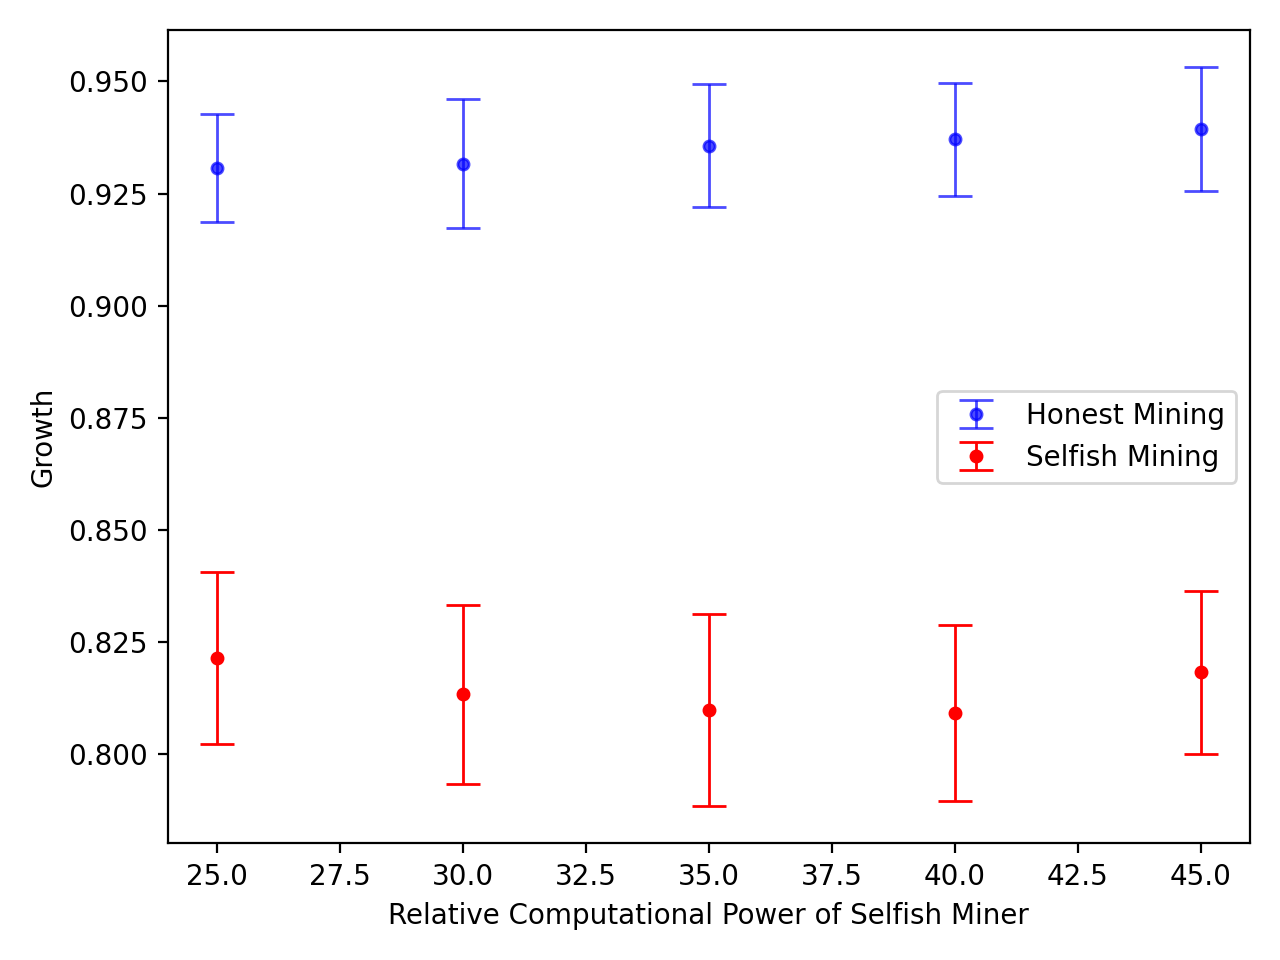
\includegraphics[width=\textwidth]{figures/growth.png}
		\caption{Relative Average Growth of Blockchain \\with Standard Deviation}
		\label{fig:multi_hr_growth}
	\end{subfigure}
	\caption{Simulations $RegRan$ Setup, multiple Hashrates, Comparison between peer with ID $0$ executing honest and selfish mining}
	\label{fig:mhr}
\end{figure}
Figure~\ref{fig:multi_hr} shows the $revenue~gain$ for relative computational power between $25\% $ and $45\% $. Figure~\ref{fig:multi_hr} shows that for selfish mining the $revenue~gain$ is on average below zero except for $45\% $ relative computational power. For honest mining it is above zero. This shows that in this scenario honest mining is outperforming selfish mining. Increasing the relative computational power also increases $revenue~gain$ for the selfish miner. The small $revenue~gain$ of the honest miner increases as well, but only very slightly. The $revenue~gain$ has a greater standard deviation for the selfish miner than for the honest miner. Especially for the selfish miner $revenue~gain$ is wide spread. Nonetheless, the results contradict the \cauth{eyal} since the authors showed a strict revenue increase for $\alpha > 33\% $. Since $\alpha$ can be seen as the fraction of blocks a miner produces it is directly linked to the relative computational power this miner possesses. Thus, according to \cauth{eyal} Figure~\ref{fig:multi_hr} should be positive for the relative compuational power greater than $33\% $, which is very clearly not the case.\\
The overall $growth$ of the blockchain is influenced by the selfish mining protocol, as is visualized in \ref{fig:multi_hr_growth}. $growth$ is the length of longest chain divided by the number of produced blocks. In an ideal case the $growth$ of the blockchain is $1$ for a complete honest network. However, network effects result in a $growth$ $~93\% $ even in a total honest network. This also explains the $revenue~gain$ of the honest miner. Since the blockchain contains forks, a peer producing a large amount of blocks will gain more revenue than its relative share. We can observe as well that selfish mining lowers the overall $growth$ of the blockchain, as expected. For the setup containing the selfish miner the overall $growth$ remains constant at around $82\% $. Note, that the $growth$ reduction seems to be independent of the relative share of computational power the selfish miner possesses, at least for relative computational powers between $25-45\% $.
Selfish mining in an homogeneous network setting does not result in a $revenue~gain$ compared to honest mining.

\subsection{Selfish Mining with Network Advantage}
Selfish Mining in a homogeneous network is not beneficial. Therefore, analysis is conducted in network settings, where the selfish miner possesses a network advantage. In the following evaluations peer with ID $0$ will possess a network advantage. This peer executes selfish and honest mining. This allows us to compare the impacts of networking advantage on honest and selfish mining. In the following experiments the selfish miner possesses a relative computational power of $45\% $.

\paragraph{Selfish Mining with Network Advantage in \textit{RegRan}}
The $RegRan$ setup utilizes a regular random graph as network topology. Increasing degree and accelerating communication process rate results in a networking advantage.
\begin{figure}[tbp]
	 \begin{subfigure}[b]{\textwidth}
		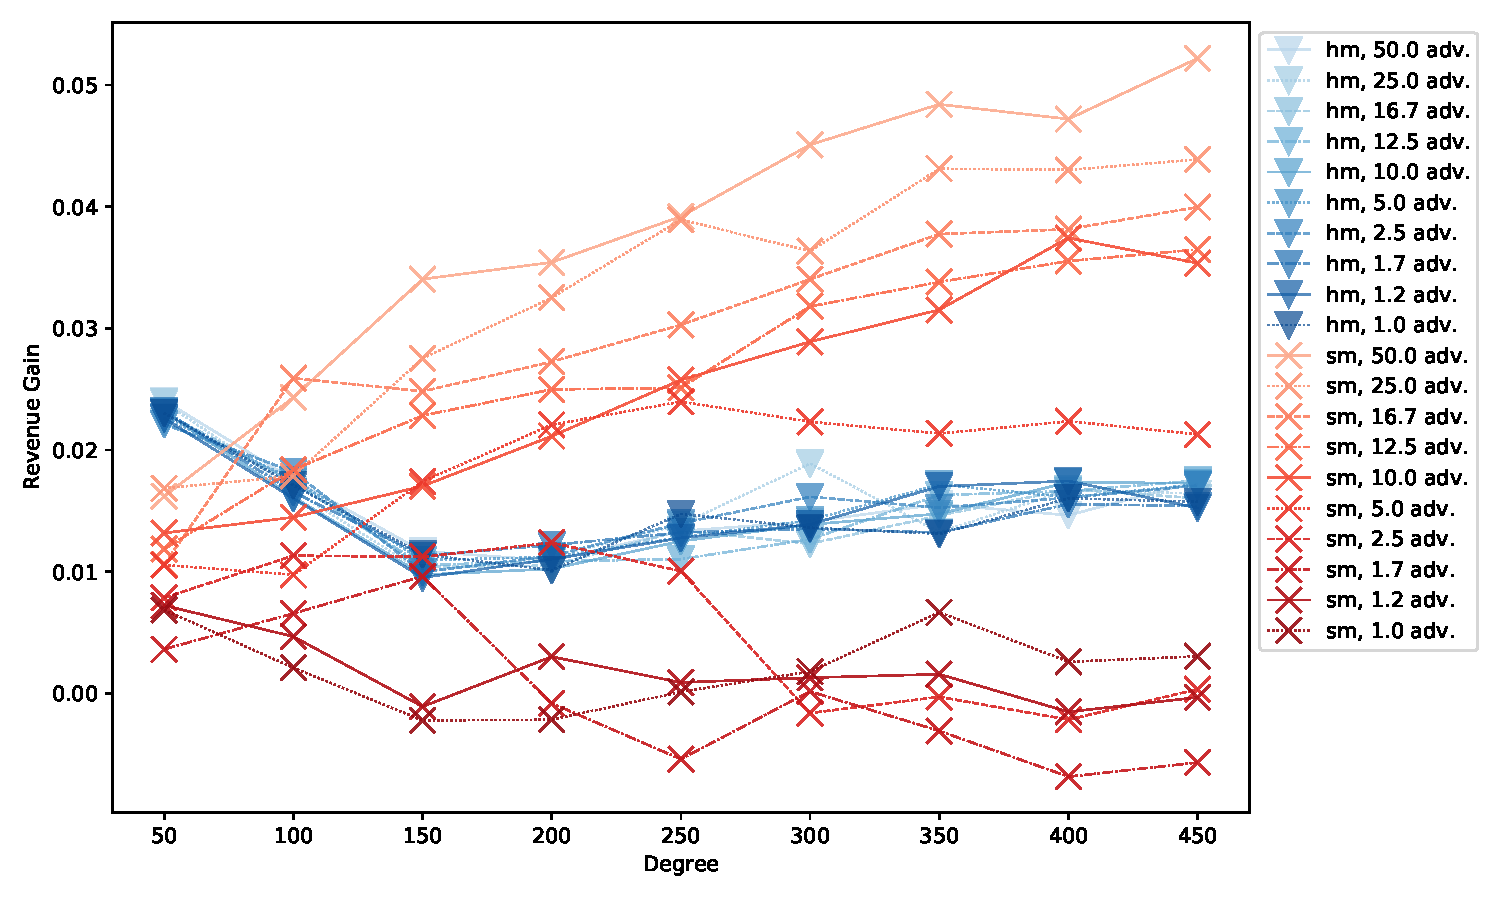
\includegraphics[width=\textwidth]{figures/sm_edge_new_revenue.pdf}
		\caption{Revenue Gain}
		\label{fig:sm_edge_rev}
	\end{subfigure}
	\hfill
	\begin{subfigure}[b]{\textwidth}
		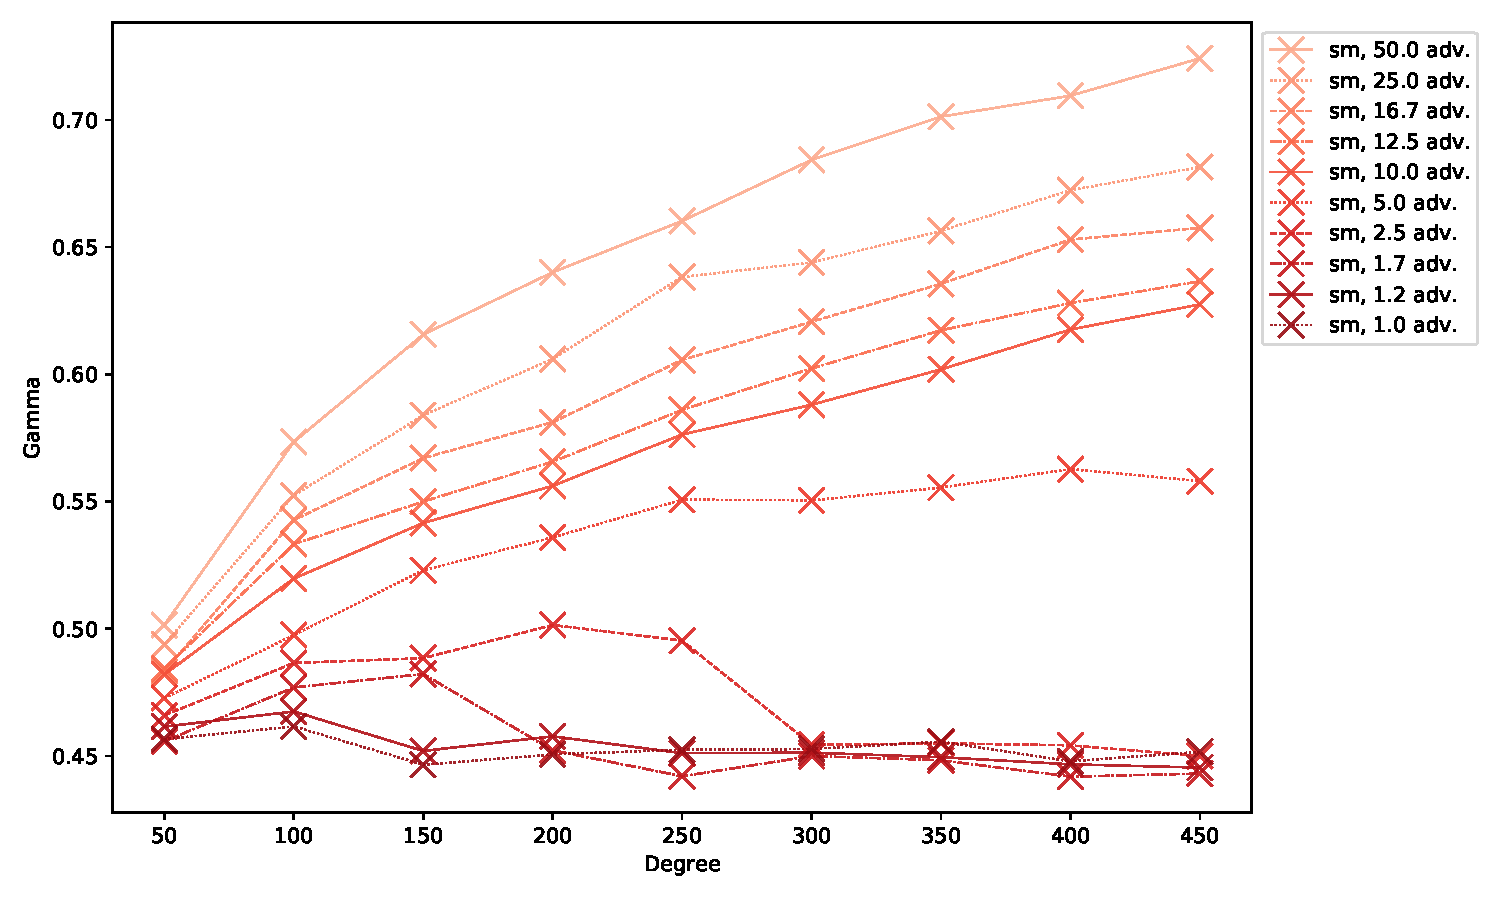
\includegraphics[width=\textwidth]{figures/sm_edge_new_gamma.pdf}
		\caption{Network Propagation Factor $\gamma_{hr}$}
		\label{fig:sm_edge_gamma}
	\end{subfigure}
		\caption{Simulations $RegRan$ Setup with Network Advantage for honest mining(hm) and selfish mining(sm), Different Communication Process Rates Advantages, $revenue~gain$ and $\gamma_{HR}$}

\end{figure}
\begin{figure}[tbp]
\begin{subfigure}[b]{\textwidth}
		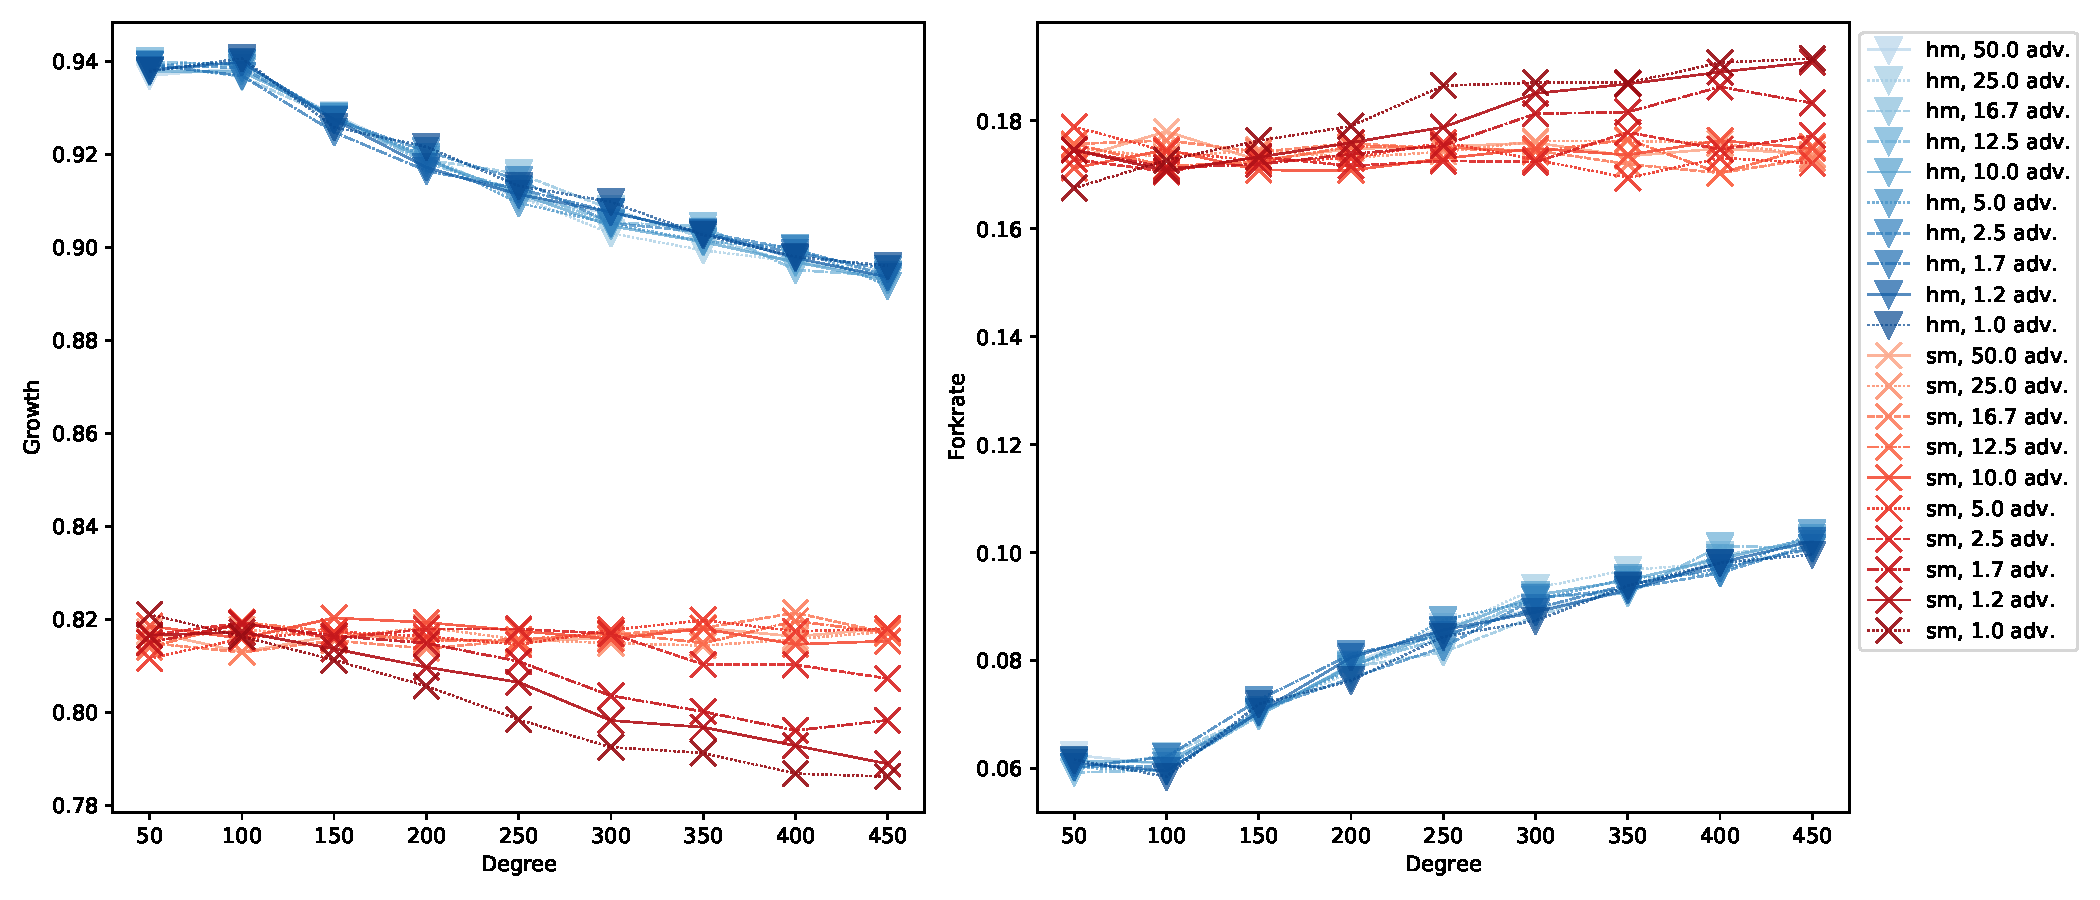
\includegraphics[width=\textwidth]{figures/sm_edge_new_growth_and_forkrate.pdf}
		\caption{Growth and Fork~rate}
		\label{fig:growth_fork}
	\end{subfigure}
\caption{Simulations $RegRan$ Setup with Network Advantage for honest mining(hm) and selfish mining(sm), Different Communication Process Rates Advantages, $growth$ and $fork~rate$}
\label{fig:sm_edge_new}
\end{figure}
Figure~\ref{fig:sm_edge_new} visualizes experiments with network advantage. We consider peer with ID $0$ executing both mining strategies and alter his network parameters. The main metric to analyze mining protocols is $revenue~gain$, which is visualized in \ref{fig:sm_edge_rev}. We can observe that selfish mining results in a more spread out $revenue~gain$ than honest mining. Additionally to an increased degree the communication process rate was increased by an advantage factor, which is shown in the legend. We can observe that for almost all cases a higher advantage factor results in more $revenue~gain$. We can also observe that increasing degree does not necessarily result in an increased $revenue~gain$, in fact it may even result in a revenue loss. This is an intuitive result since in a real system splitting bandwidth between an increasing number of connections may at one point result in an overall worse performance. However, increasing both advantage factor and degree results in an overall increased $revenue~gain$.\\
Figure~\ref{fig:sm_edge_gamma} visualizes the network propagation factor $\gamma_{hr}$. It is a metric only applicable to selfish mining, since it analyzes contest situations. It shows the fraction of the network receiving the selfish miner block before the contestant block. If we compare Figure~\ref{fig:sm_edge_gamma} and \ref{fig:sm_edge_rev} we observe a clear correlation between an increasing $\gamma_{hr}$ and $revenue~gain$. The curve for the $5$-times advantage factor even visualizes that if $\gamma_{hr}$ stagnates, the $revenue~gain$ does so as well. The $2.5$-times advantage factor curve shows at $300$ degree, that if $\gamma_{hr}$ drops significantly below $50\% $, the selfish mining $revenue~gain$ drops below the honest mining $revenue~gain$.\\
Honest mining is mostly unaffected by changes in advantage factor, but very much affected by changes to the degree of the miner. However, in comparison to the $revenue~gain$ of the selfish miner the honest miner $revenue~gain$ is quite constant. The honest miner shows the highest $revenue~gain$ for a degree less than the network average. This $revenue~gain$ quickly decreases until $150$ were it starts increasing again. If we observe $growth$ and $fork~rate$ in Figure~\ref{fig:growth_fork} we can see that for the degree $50$ and $100$ the $growth$ of the blockchain is the highest and constant for the honest miner scenarios. For degrees larger than $100$ the $growth$ starts rapidly decreasing. We observe the inverse behavior for the $fork~rate$. Since the $fork~rate$ is close to $1-growth$ the forks are very small and we can not observe a network consensus partition. For a degree greater than $150$ we can find a relationship between increasing $revenue~gain$ due to decreasing $growth$. Since the relative computational power of the miner is $45\% $ he profits from a decreased $growth$. However, the increased $revenue~gain$ for degree $50$ and $100$ with a relatively high $growth$ of $94\% $ implies that there exists a $growth$ threshold were the honest miner benefits from a better growth. We presume, that relatively more of his blocks are included in the blockchain if the growth surpasses a certain threshold.\\
The selfish miner scenarios show mostly a very similar low $growth$ and high $fork~rate$. For lower advantage factors $growth$ decreases correlate to a decreased $revenue~gain$. This is most likely due to the fact, that the selfish miner can not effectively push his blocks in the main chain of the blockchain, resulting in a decreased $growth$ and increased $fork~rate$. However, independent of mining strategy we observe $fork~rate \approx 1-growth$ which implies that for both mining strategies we only observe small forks.

\paragraph{Selfish Mining with Network Advantage in \textit{ScaFre}}
The $ScaFre$ setup utilizes a scale free graph as network topology, implying that node degrees are exponentially distributed. To achieve a network advantage for peer with ID $0$, we removed the edges, that were constructed through the Barabasi-Albert Algorithm and then connected peer with ID $0$ to a new amount of peers. The strategies to connect peer with ID $0$ are uniformly at random and according to betweenness centrality. Betweenness centrality is a measure to express how central a node is in a given graph. It is the number of shortest paths that pass through the node\cite{bcent}.
\begin{figure}[tbp]
	 \begin{subfigure}[b]{\textwidth}
		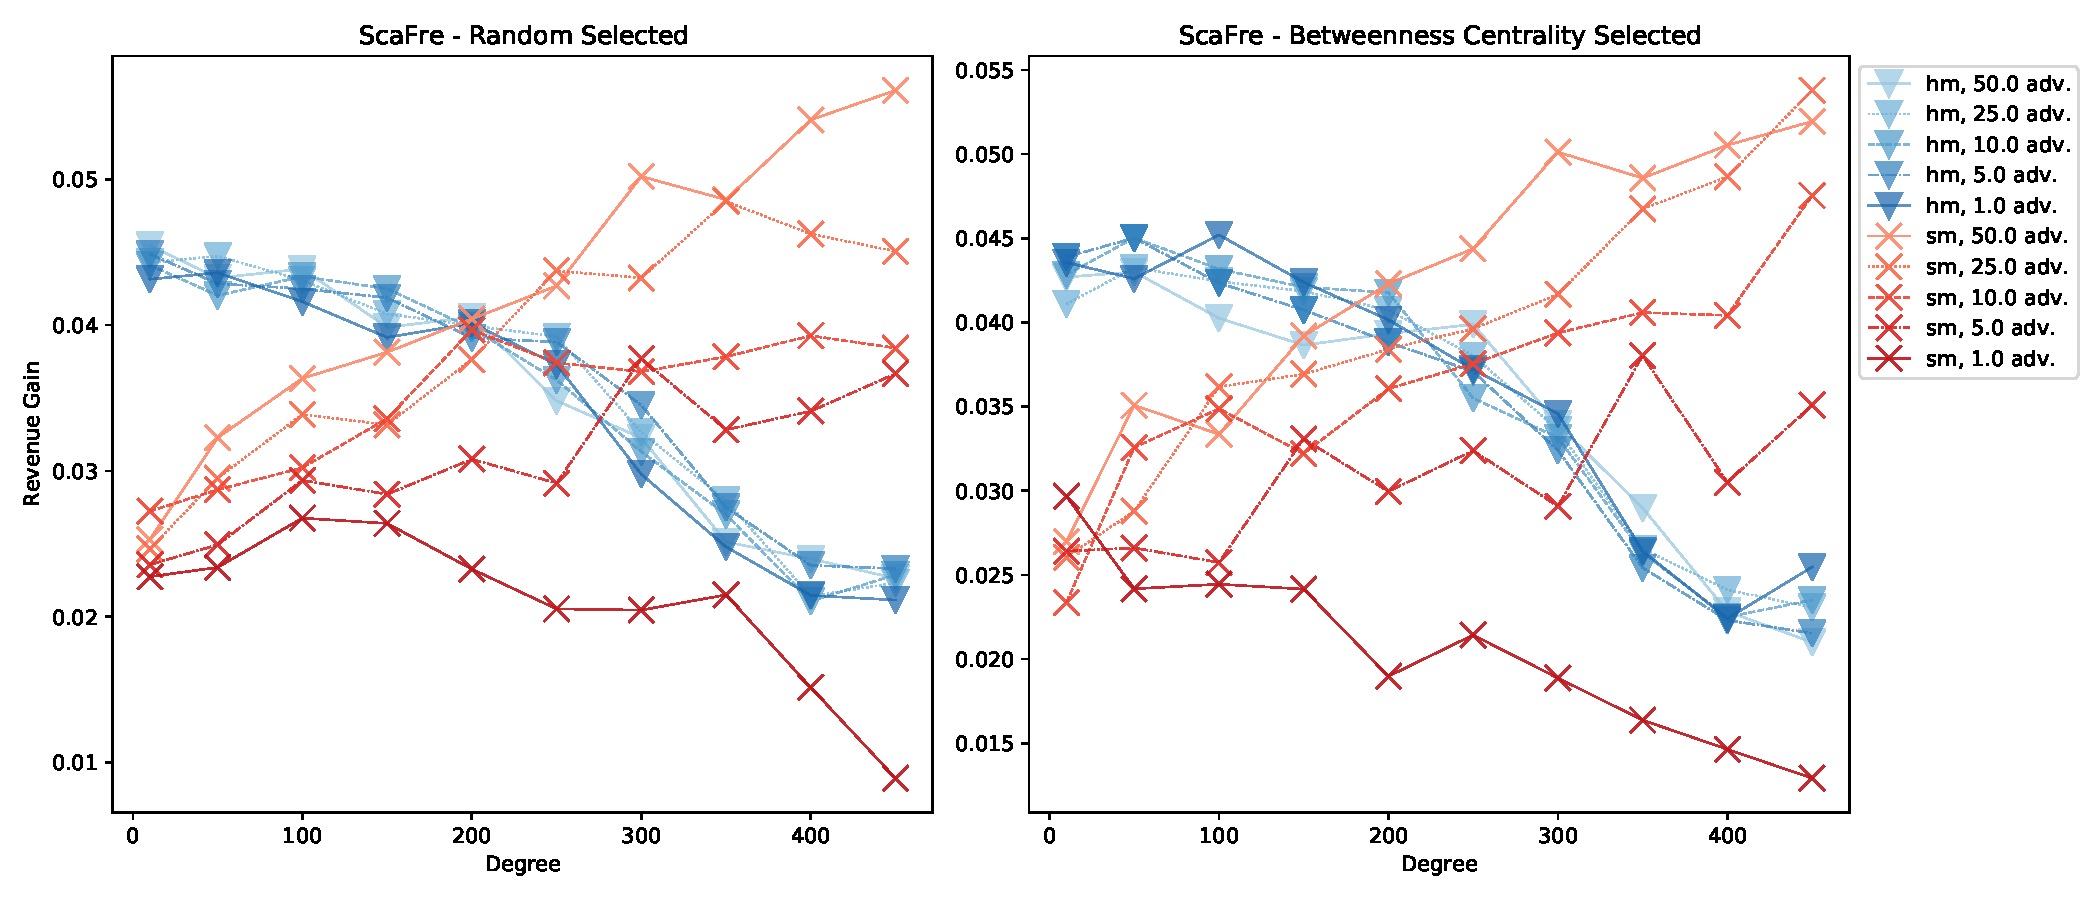
\includegraphics[width=\textwidth]{figures/sm_edge_revenue_barabasi.pdf}
		\caption{Revenue Gain}
		\label{fig:sm_edge_rev_bara}
	\end{subfigure}
	\begin{subfigure}[b]{\textwidth}
		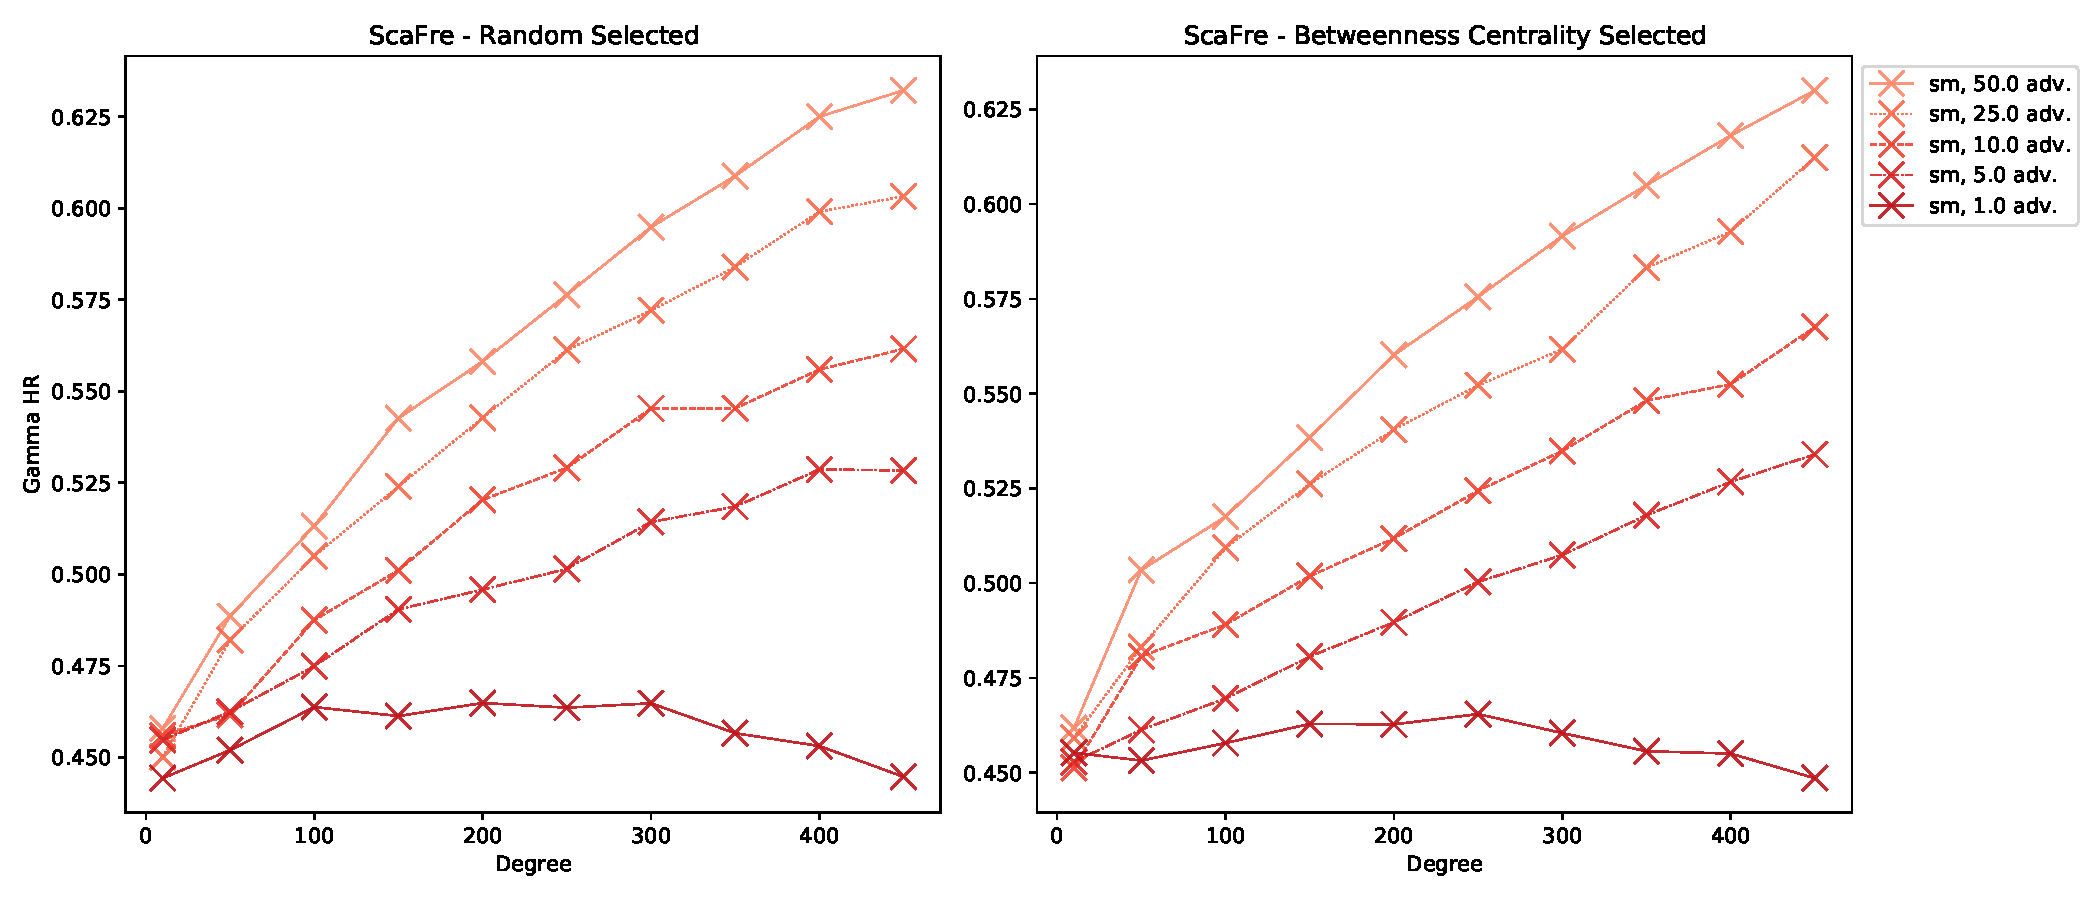
\includegraphics[width=\textwidth]{figures/sm_edge_gamma_barabasi.pdf}
		\caption{Network Propagation Factor $\gamma_{hr}$}
		\label{fig:sm_edge_gamma_bara}
	\end{subfigure}
	
	\caption{Simulations $ScaFre$ Setup with Network Advantage for honest mining(hm) and selfish mining(sm), Different Communication Process Rates Advantages, $revenue~gain$ and $\gamma_{HR}$}
\end{figure}
\begin{figure}[tbp]
\begin{subfigure}[b]{\textwidth}
		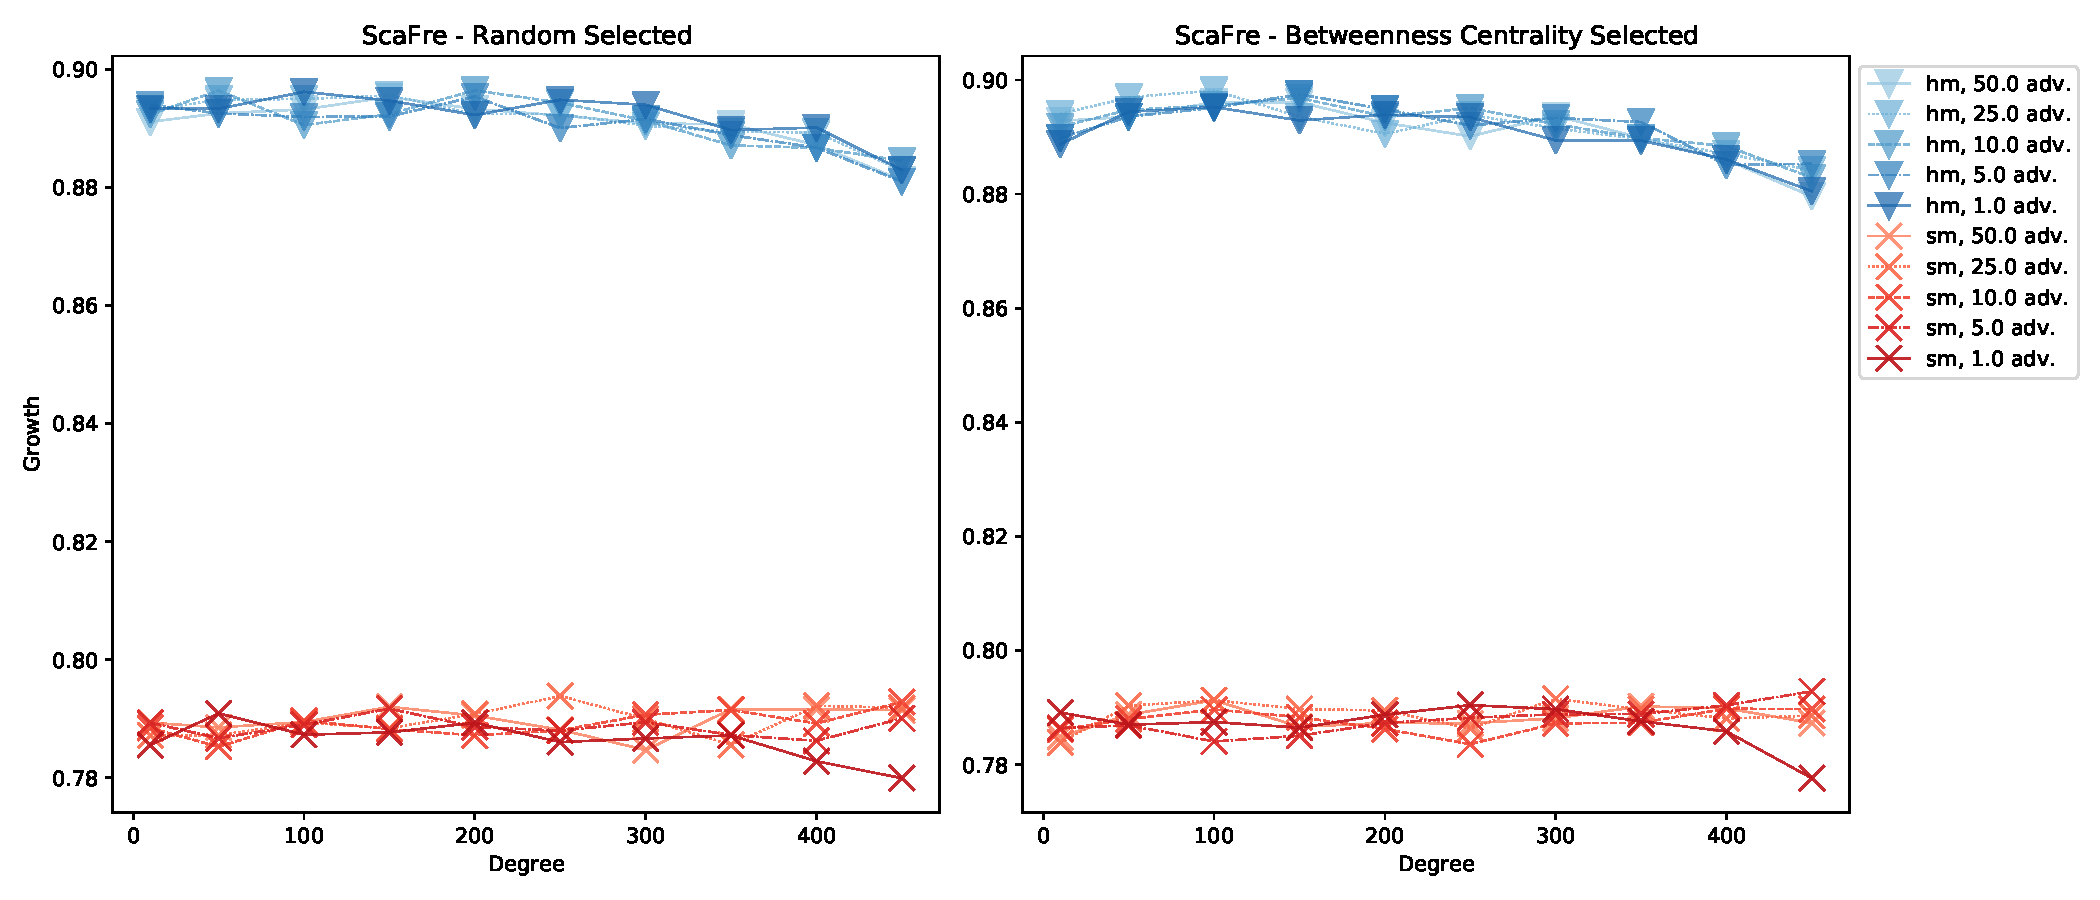
\includegraphics[width=\textwidth]{figures/sm_edge_growth_barabasi.pdf}
		\caption{Growth}
		\label{fig:growth_bara}
	\end{subfigure}
	\begin{subfigure}[b]{\textwidth}
		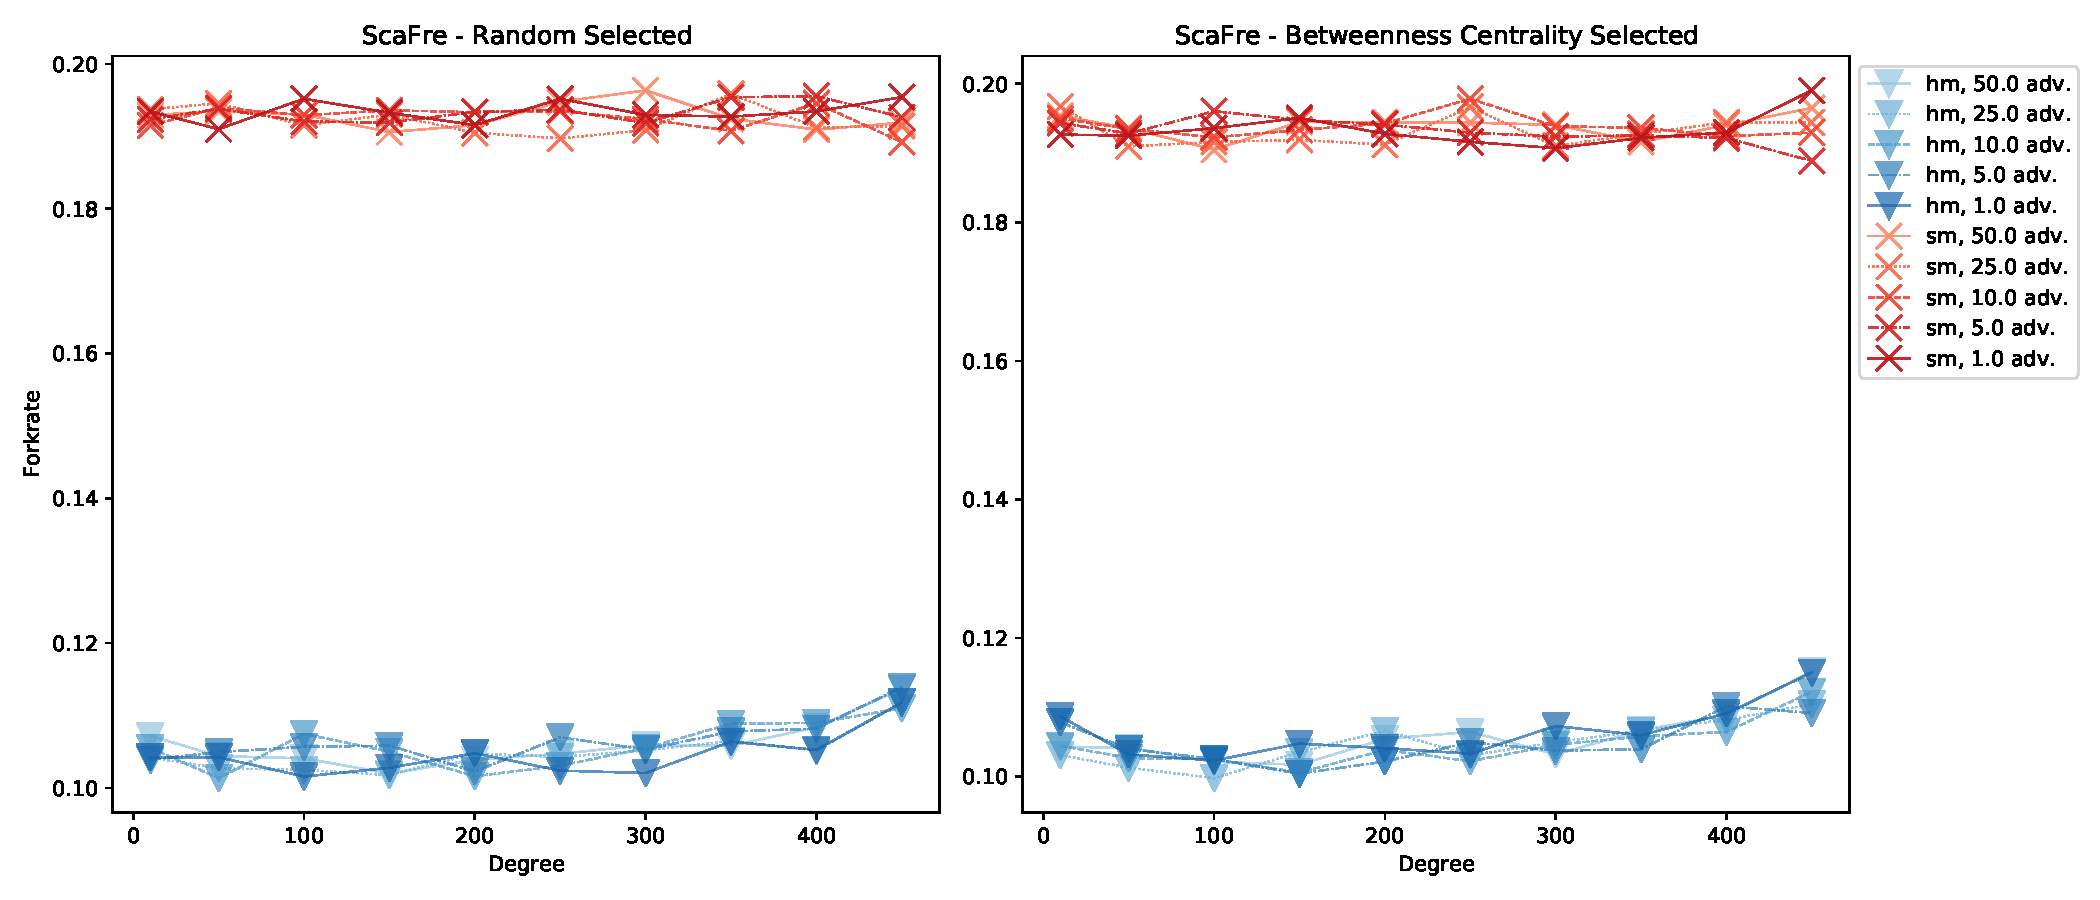
\includegraphics[width=\textwidth]{figures/sm_edge_forkrate_barabasi.pdf}
		\caption{Fork Rate}
		\label{fig:fork_bara}
	\end{subfigure}
\caption{Simulations $ScaFre$ Setup with Network Advantage for honest mining(hm) and selfish mining(sm), Different Communication Process Rates Advantages, $growth$ and $fork~rate$}
\label{fig:sm_edge_barabasi}
\end{figure}\\
Figure~\ref{fig:sm_edge_barabasi} visualizes the results of network advantage simulations carried out in the $ScaFre$ parameter setup. Overall we cannot observe a major difference between the measured metrics in Figure~\ref{fig:sm_edge_barabasi} between both peer selection strategies. Figure~\ref{fig:sm_edge_rev_bara} shows the $revenue~gain$ for honest mining and selfish mining for both strategies. For selfish mining we see a similar dependence of $revenue~gain$ to increasing degree and communication process rate advantage as in the $RegRan$ setup. Selfish mining results in a more spread out $revenue~gain$ than honest mining. An increase in both degree and communication process rate results in a higher revenue gain. If degree and communication process rate surpass a certain threshold, selfish mining produces more revenue gain than honest mining. This threshold is at least a 30-times faster communication process rate and a degree of 250 or higher for both strategies.\\
We also see the same clear correlation between an increasing $\gamma_{hr}$ and $revenue~gain$. A $\gamma_{hr}$ significantly higher than $50\% $ results in a significant $revenue~gain$ for the selfish miner. As expected the highest $\gamma_{hr}$ results in the highest $revenue~gain$ for the selfish miner.\\
A major difference to the $RegRan$ setup is the $revenue~gain$ of the honest miner in the $ScaFre$ setup. The honest miner has a very high $revenue~gain$ with low degrees, which decreases as degree increases. This is in contrast to the $RegRan$ experiments where  $revenue~gain$ remained quite constant with changing degrees for the honest miner. However, in both setups $revenue~gain$ for the honest miner is independent of communication process rate advantage. We observe the highest $revenue~gain$ of $~0.045$ to be at 10-degrees for the honest miner.\\
Figure\ref{fig:growth_bara} and Figure\ref{fig:fork_bara} visualize both $growth$ and $fork~rate$. Both metrics are quite constant for both peer selection strategies and as expected selfish mining leads to a lower $growth$ and higher $fork~rate$. Additionally changes in degree as well as communication process rate advantage do not change $growth$ or $fork~rate$ significantly. This is true for both peer selection strategies and for selfish mining as well as honest mining. Compared to $RegRan$, $ScaFre$ experiments seem to have an overall lower $growth$ and higher $fork~rate$. The relationship of $fork~rate \approx 1-growth$ remains. Communication process rate advantage changes result in a more spread out $growth$ and $fork~rate$ for selfish mining in the $RegRan$ setup. However, this behavior is not visible in the $ScaFre$ setups.\\
\subsection{Communication Rate Distribution and Bottlenecks}
The question remains why honest mining results for low degrees in such a high $revenue~gain$ and drops for higher degrees. An overall revenue gain of the honest miner can be attributed to the low $growth$ of the blockchain. However, since $growth$ remains constant it can not be correlated to changing $revenue~gain$.
\begin{figure}[tbp]
	\begin{subfigure}[b]{\textwidth}
		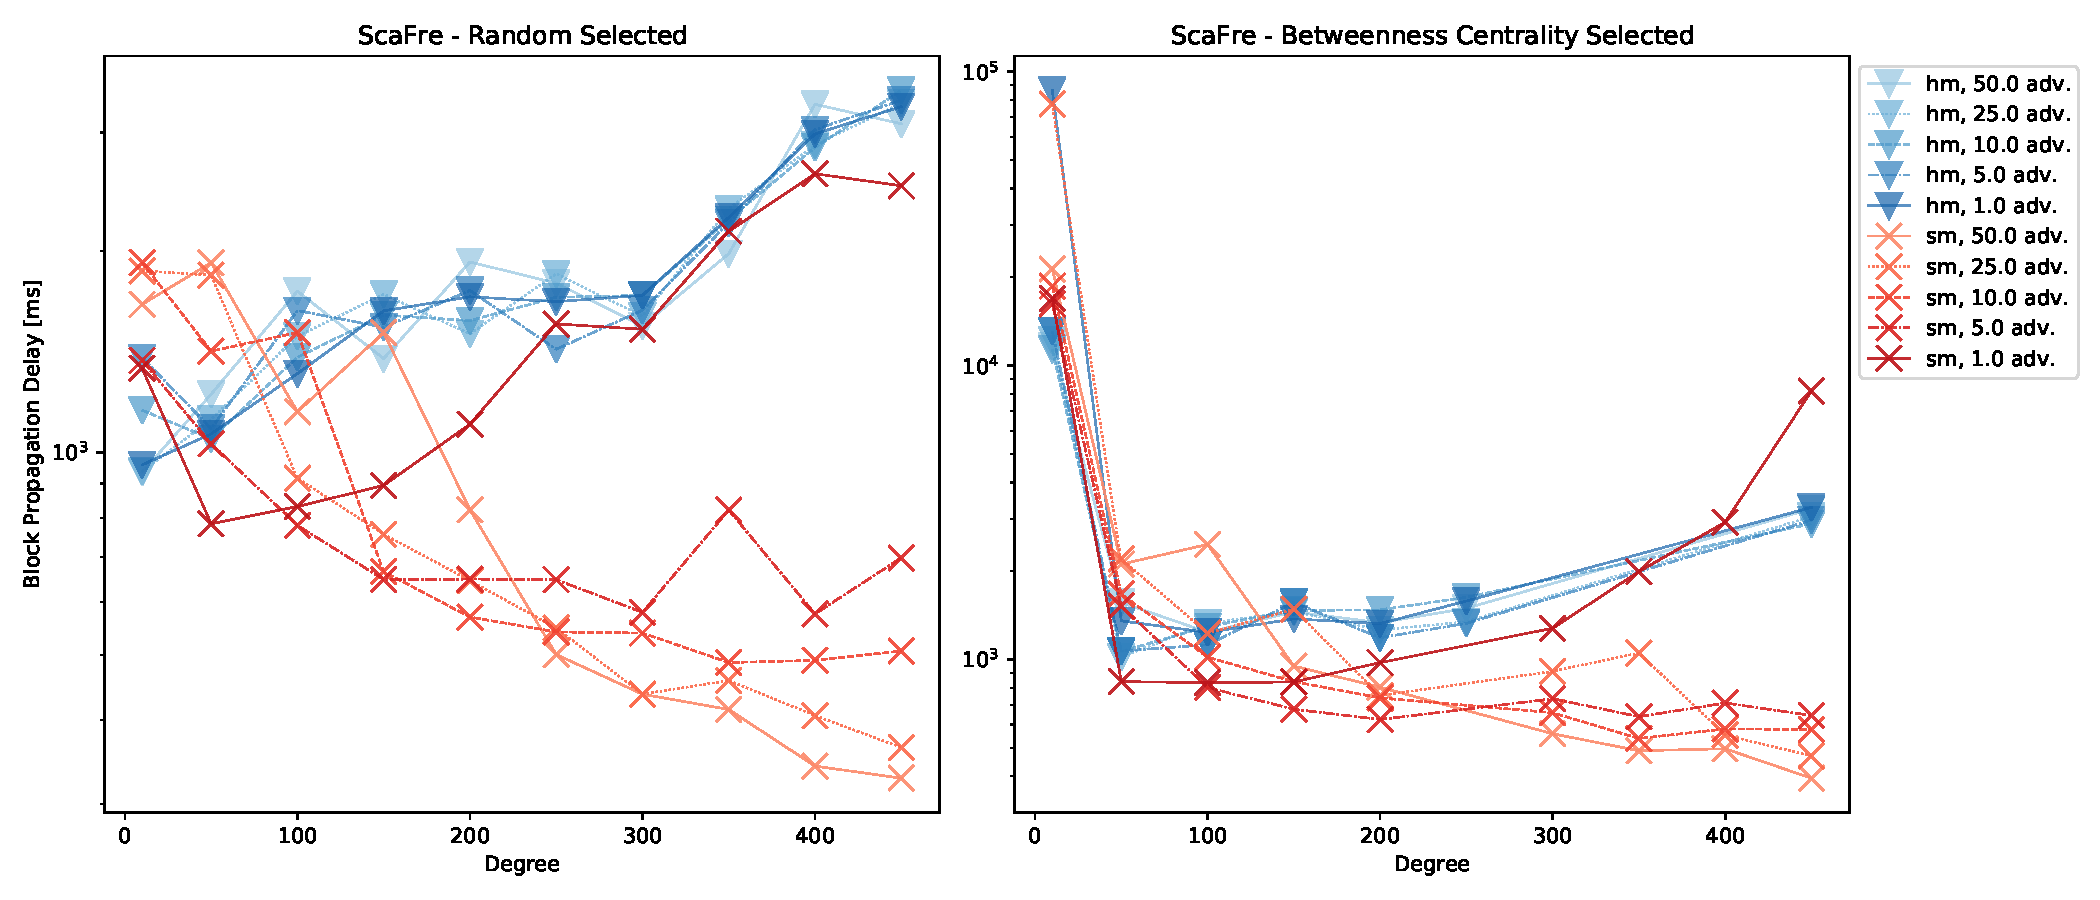
\includegraphics[width=\textwidth]{figures/sm_edge_block_scafre.pdf}
		\caption{$ScaFre$ simulation setup}
		\label{fig:blockprop_bara}
	\end{subfigure}
	\begin{subfigure}[b]{\textwidth}
		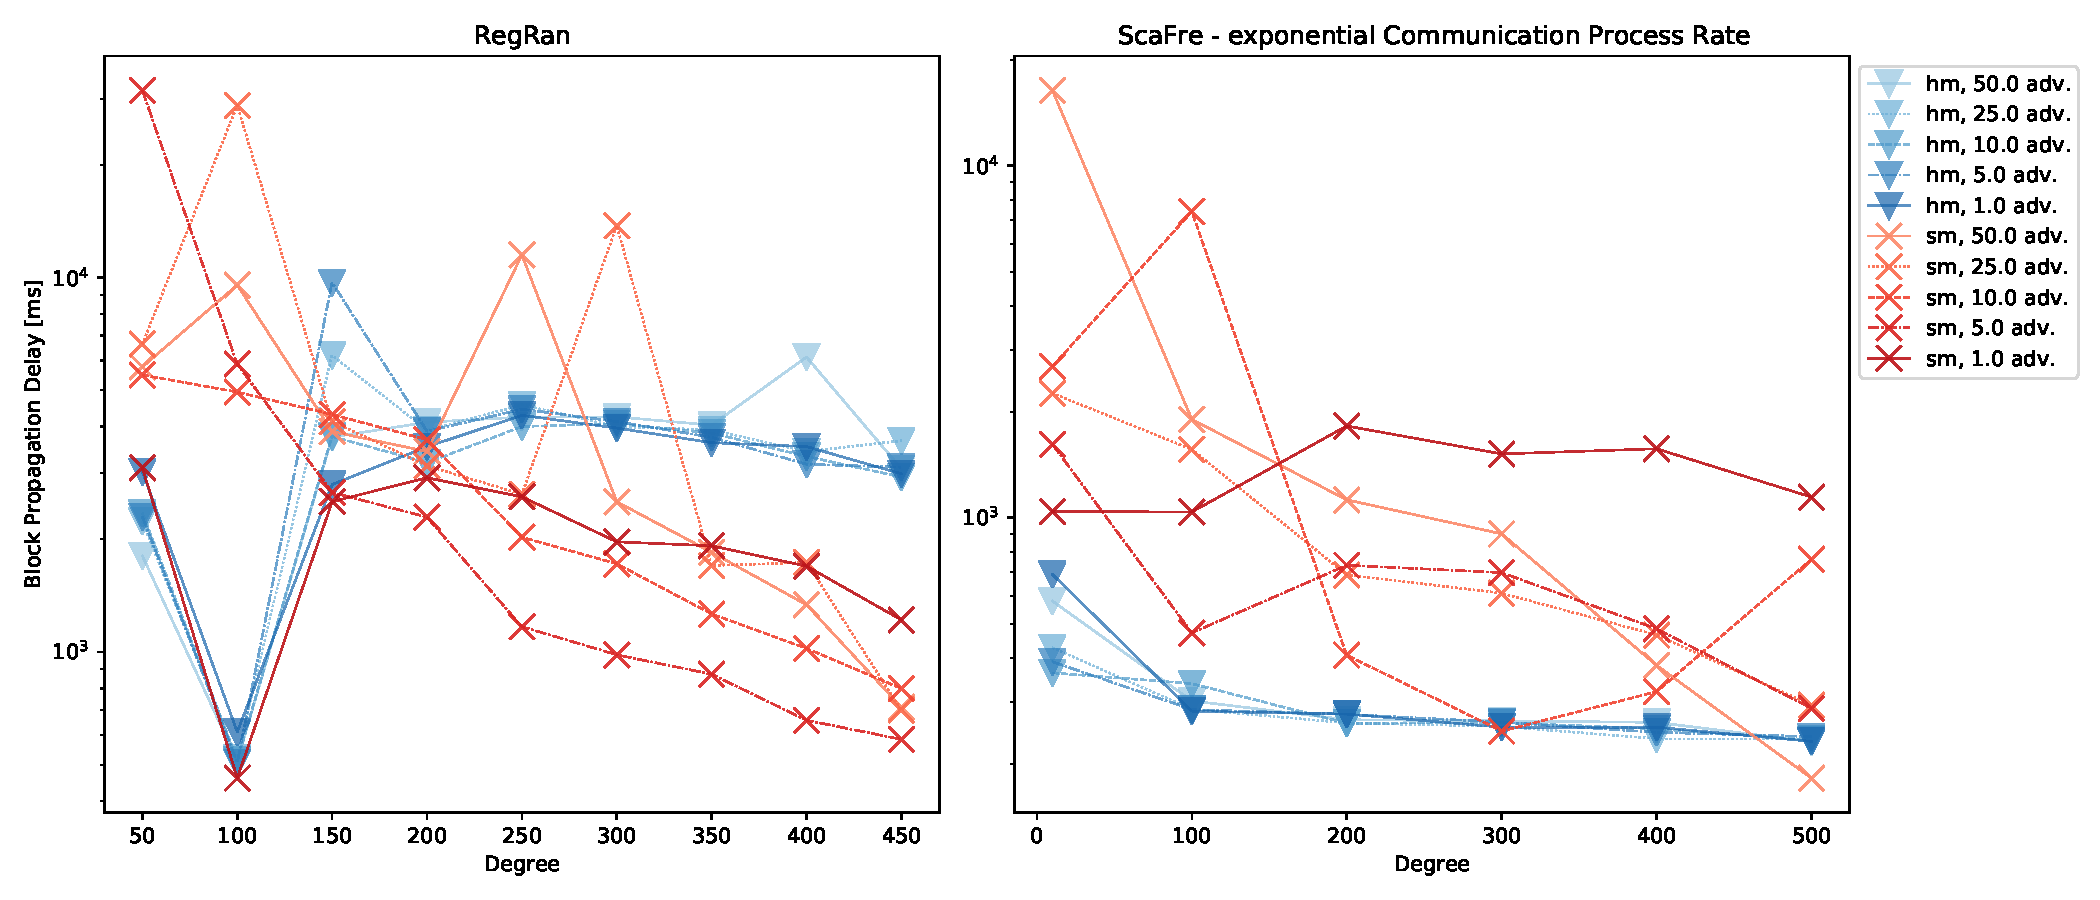
\includegraphics[width=\textwidth]{figures/sm_edge_block_prop_rr_and_bc_dc.pdf}
		\caption{$RegRan$ and $ScaFre$- exponential distributed communication process rate simulation setup}
		\label{fig:blockprop_2}
	\end{subfigure}
\caption{Block Propagation delay of Blocks mined by peer with ID $0$}
\label{fig:blockprops}
\end{figure}\\
Figure\ref{fig:blockprop_bara} shows the  block propagation delay of blocks mined by peer with ID $0$ for the $ScaFre$ simulation setup. Especially for honest mining we can see an increasing block propagation delay for an increasing degree. Since blocks of peer with ID $0$ need more time to propagate through the network it is less likely that those blocks will be part of the main chain. This results in a revenue loss. For selfish mining we observe a similar behavior. Selfish mining with no communication process rate advantage shows the least amount of revenue gain. We also observe a very high block propagation delay for 10-degree in the betweenness centrality selected simulations. We deduce that high centrality peers in this setup are a bottleneck. In the $ScaFre$ setup every peer has the same average communication process rate. This results in a higher average time to cover all edges for a peer with a higher degree. Thus, this peer becomes a bottleneck and it is not beneficial to connect to those peers with the highest centrality. This also explains why it is beneficial for the selfish miner to have a higher degree once he has a communication process rate advantage, since then he can effectively use multiple parallel paths to propagate his blocks faster. We also see this behavior in Figure~\ref{fig:blockprops} since for communication process rate advantages and higher degrees the selfish miner achieves lower block propagation delays.\\
For the $RegRan$ block propagation delays we observe a more diverse picture. For an increased degree and communication process rate advantage we observe lower block propagation times for the selfish miner. For the honest miner we observe the minimal block propagation at 100-degrees. The overall block propagation delay is higher than in the $ScaFre$ experiments for the honest miner, which would explain the reduced revenue gain. This leads to the assumption that for honest mining a lower block propagation delay is correlated to a higher revenue gain.\\
Figure~\ref{fig:blockprop_2} visualizes the block propagation delay for a modified $ScaFre$ setup. In $ScaFre$ node degrees are exponentially distributed, but the communication process rate is constant. To further evaluate if central nodes become bottlenecks the modified $ScaFre$ setup scales communication process rate distribution to degree distribution. A high degree node with the same communication process rate as a low degree node needs more time to cover all of his connections. The modified $ScaFre$ setup scales communication process rates in such a way, that the average round trip time remains the same, independent of node degree.
\begin{figure}[tbp]
	\begin{subfigure}[b]{\textwidth}
		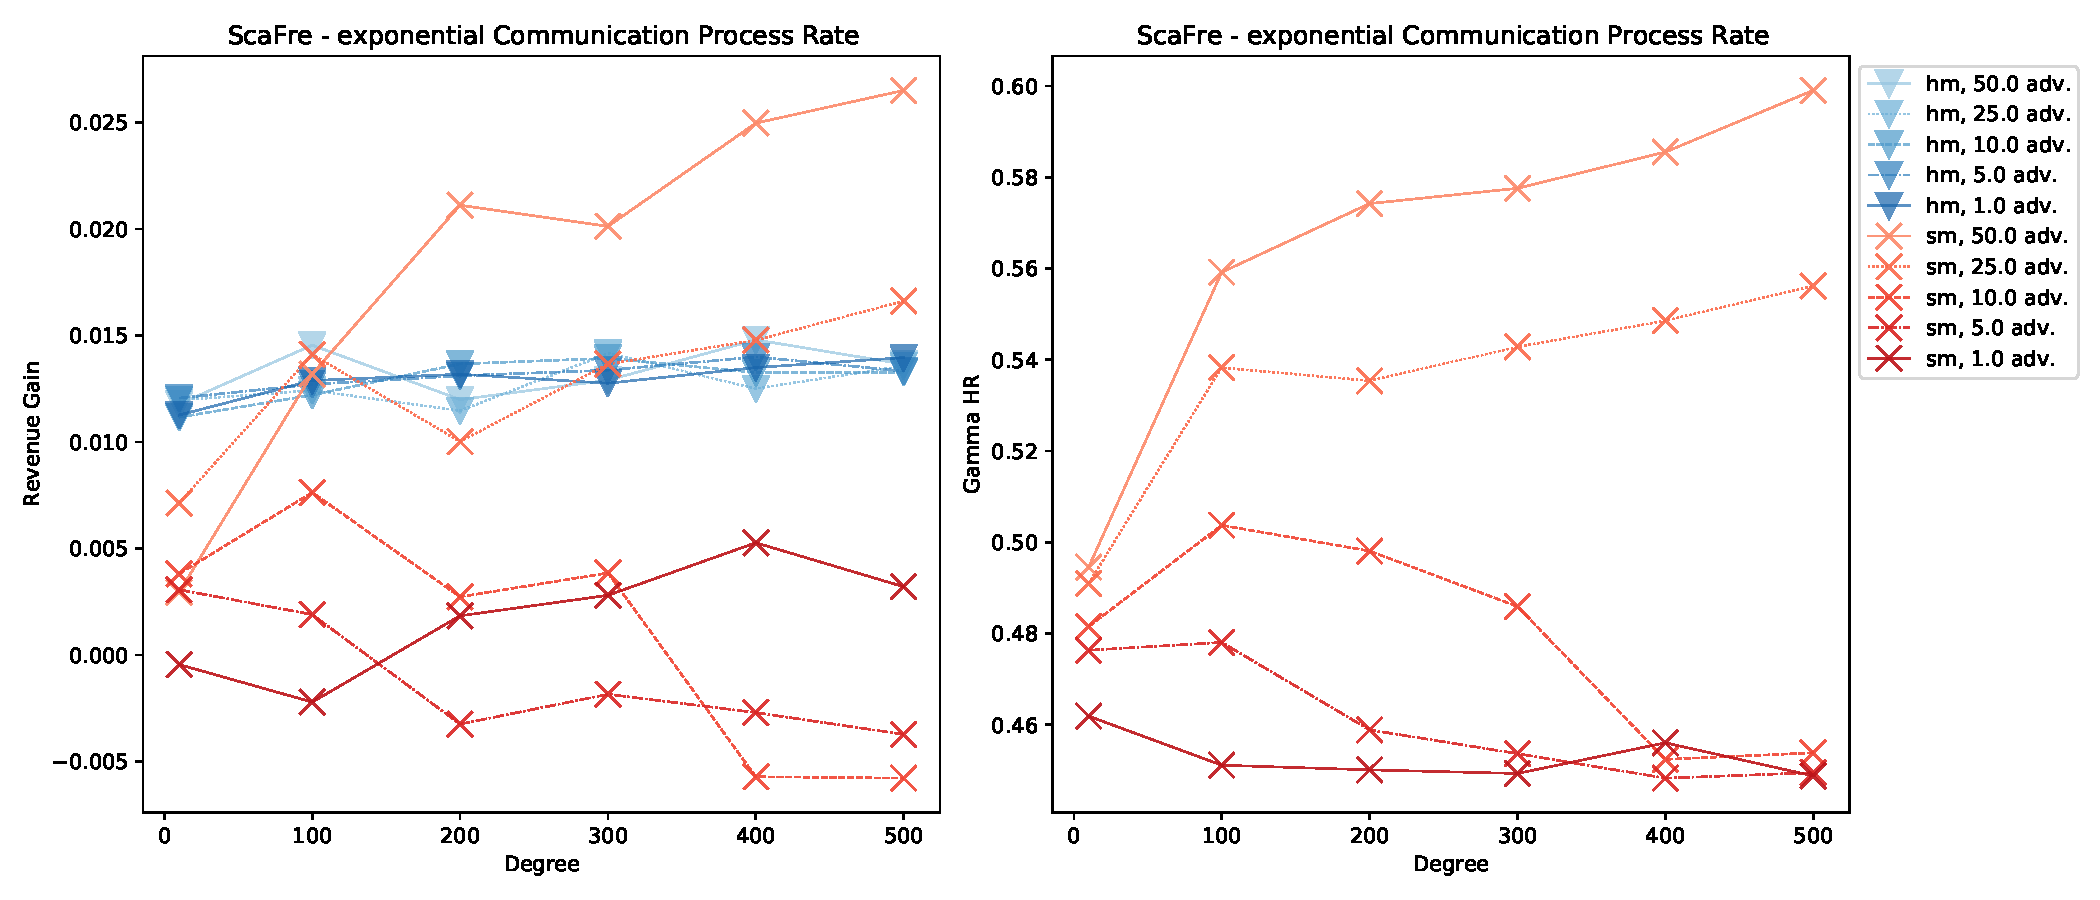
\includegraphics[width=\textwidth]{figures/revenue_gamma_barabasi_bc_dc.pdf}
		\caption{Revenue Gain and Gamma}
		\label{fig:revgain_bc_dc}
	\end{subfigure}
	\begin{subfigure}[b]{\textwidth}
		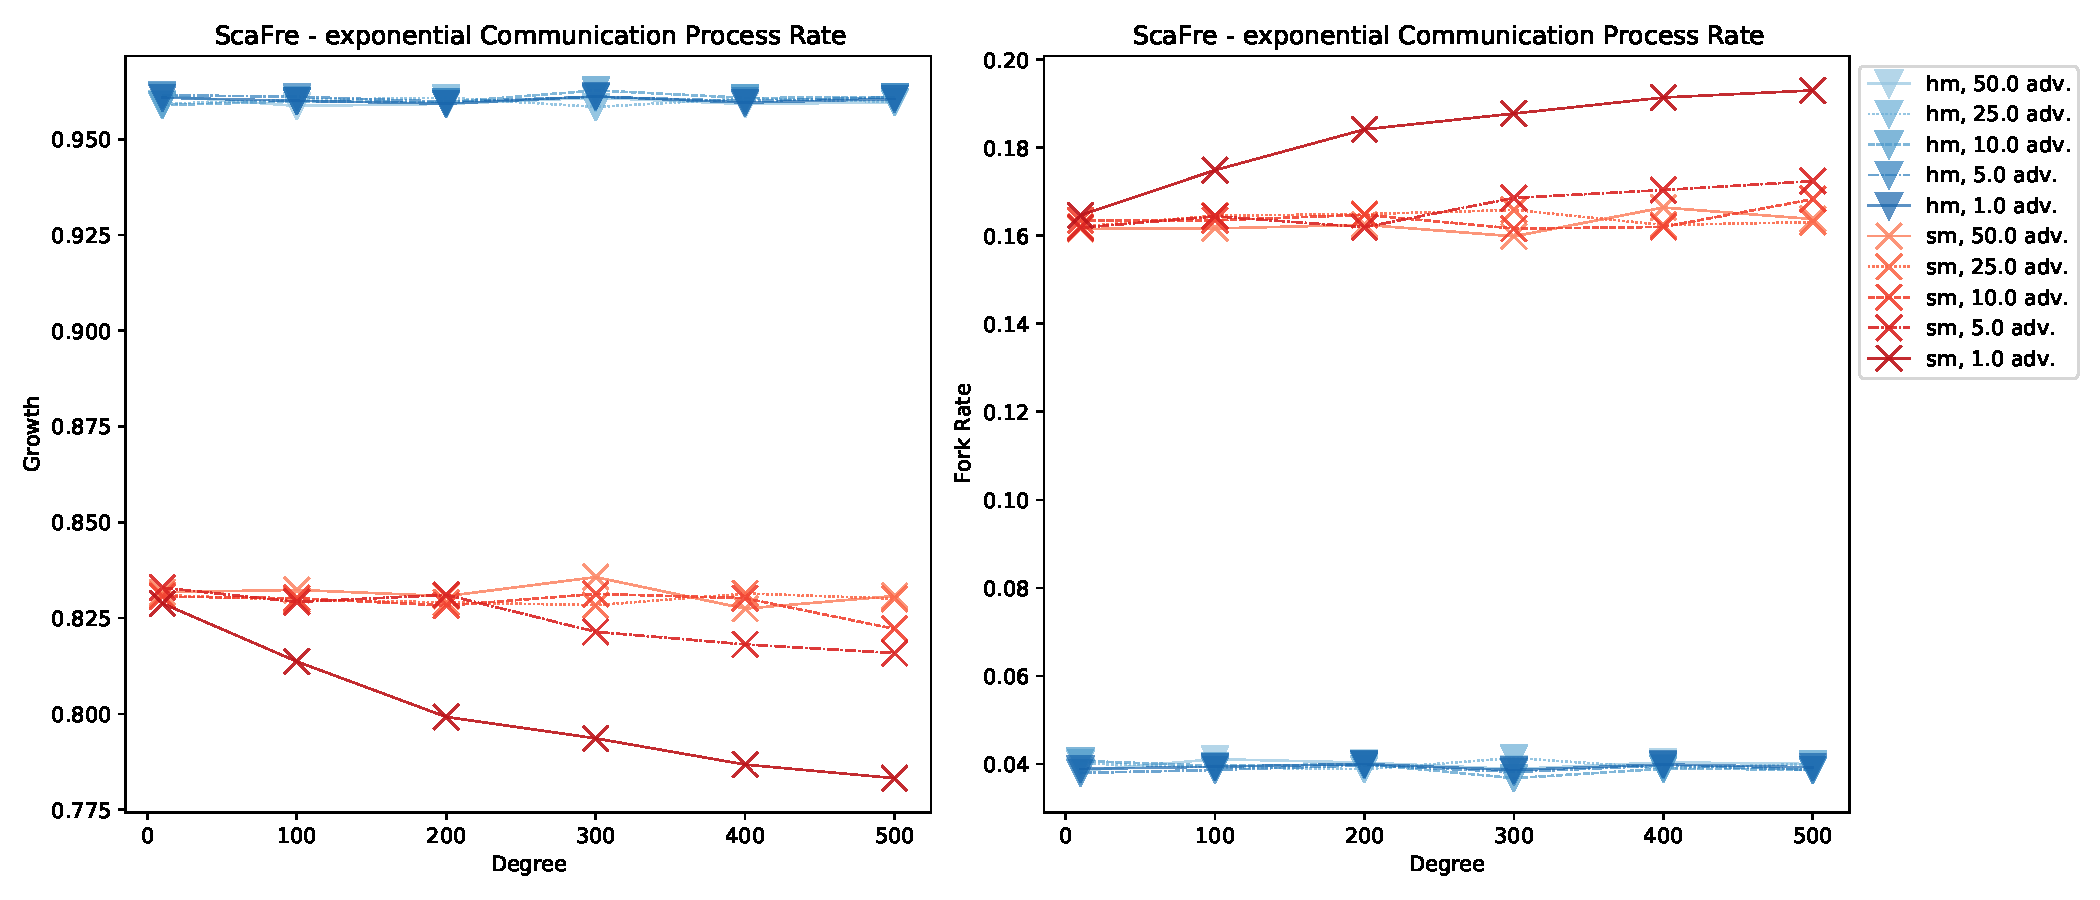
\includegraphics[width=\textwidth]{figures/growth_forkrate_barabasi_bc_dc.pdf}
		\caption{Growth and Forkrate}
		\label{fig:growth_bc_dc}
	\end{subfigure}
\caption{Simulations $ScaFre$ with exponential Communication Rate Distribution Setup with Network Advantage for honest mining(hm) and selfish mining(sm), Different Communication Process Rates Advantages}
\label{fig:bc_dc}
\end{figure}\\
Figure~\ref{fig:blockprop_2} shows the block propagation delay for peer with ID $0$ in this modified topology. We observe that the honest miner can transmit his blocks faster. Overall the system seems more stable since $growth$ is higher than in $RegRan$ and $ScaFre$ and the $fork~rate$ is lower. This is visualized in \ref{fig:growth_bc_dc}. Figure~\ref{fig:revgain_bc_dc} visualizes $revenue~gain$ and $\gamma_{HR}$. The honest miner has a lower and constant $revenue~gain$ compared to previous experiments. This in conjunction with the higher $growth$ implies that the network is more stable in this modified version. The selfish miner experiences a lowered $revenue~gain$ as well. However, we do not observe lower values of $\gamma_{HR}$. The reduced $revenue~gain$ must therefore be a result of the increased $growth$ and reduced $fork~rate$. This seems intuitive because as stated by \cauth{eyal} selfish mining benefits from an increased number of forks.\\
To sum up we observe major key relations between different system parameters. Selfish mining does in fact produce an increased revenue if network advantage and relative hashrate exceed a certain threshold. In fact we observe a revenue gain up to $0.052$ for a high network advantage. For a relative hashrate of $45\% $ we observe the needed network advantage to consist of an increased bandwidth by a factor 5 to 25 and the ability to establish more connections. The actual threshold highly depends on the topology and overall characteristic of the rest of the network. We observe that selfish mining is more effective in a system with a reduced growth of the blockchain. Additionally a relationship of $growth \approx 1-fork~rate$ is clearly visible, which implies that forks mainly consist of 1 block. Honest mining produces an increased revenue as well. For the tested high relative hashrate of $45\% $ honest mining produced a revenue gain between $0.01$ and $0.045$. Additionally we see that the produced revenue of honest mining highly depends on the performance of the rest of the network. This is in contrast to selfish mining. While selfish mining also depends on the rest of the network, revenue can increase by increasing bandwidth and degree of the selfish miner. Overall we see a high dependence between the performance of selfish mining and network advantage of the peer executing the attack.\\
From a more general point of view we see that revenue does not solely depend on relative hashrate. It is a combination of relative hashrate, selected mining strategy and network characteristics. The selected mining strategy is influenced by different network effects. Honest mining is strongly influenced by the overall network and can produce revenue gain. Selfish mining is strongly influenced by the network advantage a peer possesses. Without a high hashrate and network advantage selfish mining is outperformed by honest mining. However, we observe that selfish mining can outperform honest mining with a high enough relative hashrate and network advantage.









 

\chapter{Related Work}\label{chap:relatedwork}
Selfish mining is a statistical attack. In order to analyze profit, it is therefore beneficial to analytically model selfish mining. Moreover to study the impact of deviating mining strategies and gain realisitic resulsts, it is very important to represent the blockchain network as close to reality as possible in a mining model. In the following recent selfish mining models as well as network models will be discussed.


\section{Selfish Mining Models}
Proof-of-work Mining is most commonly modelled through Markov decision processes.
It is generally used to model decision making, where the outcomes are influenced by random processes and the decision of the decision maker~\cite{ibe2013markov}.
In the case of selfish mining controls his decision making process and for the rest of the network, the block arrival and block propagation is modelled through stochastic processes. Once implemented, a Markov model can be used to analytically estimate system properties. Selfish mining is concerned with maximizing obtained mining rewards, which is also called revenue.

\citeauthor{eyal} first described a selfish mining model based on Markov decision processes~\cite{eyal}.
They ran simulations to estimate revenue gain. Since blockchain systems use a peer-to-peer network to propagate mined blocks, it is important to analyze how the network was implemented in this model. Block propagation time is considered negligible compared to block generation time~\cite{eyal}. As a result, \citeauthor{eyal} consider communication to be instantaneous~\citep{eyal}. They found that selfish mining increases profitiability for a relative mining power greater than $25\%$ compared to the network.

\citeauthor{optimal_sm} further extended the model to consider all possible actions a selfish miner can perceive. Block propagation time remains unassessed, since it is again considered to be much smaller than block generation time.  \citeauthor{optimal_sm} again utilize Markov decision processes to model the system. They find a number of optimal policies and provide an analysis on the upper bound of revenue increase through selfish mining strategies.
This Markov model was widely used and adopted in other research directions studying other aspects of selfish mining. For example, the behavior of multiple selfish miners was simulated through \citeauthor{multi_sm}~\cite{multi_sm}. One of the main findings is that the lower bound on the profitability treshhold decreases with the number of selfish miners.
\citeauthor{deepDiveSM}~\cite{deepDiveSM} extended the model of \citeauthor{optimal_sm}~\cite{optimal_sm} even further to analyze multiple selfish miners. This resulted in a more complex state space of the markov decision process. They show that in fact for the symmetric selfish miner, i.e. all selfish miners have the same hashrate, the profitability threshhold decreases, but for the asymmetric case the threshhold increases. The focus of this research was to deepen the understanding of different selfish mining strategies. However, networking factors remained unassessed.

\citeauthor{xiao_modeling} study the impact on the profitability threshhold and revenue gain of a networking advantage possessed by the selfish miner~\cite{xiao_modeling}. They model the network as a graph and find that networking advantage correlates to the betweenness centrality of the selfish miner. Additionally it highly affects the profitability threshhold and revenue gain of the attacker. This indicates that the structure of the network influences the selfish mining strategy. However, this model remains very abstract, since only the peer-to-peer layer and structure is modelled as a graph, disregarding any limitations imposed by physical infrastructure such as bandwidth. Nonetheless, it indicates that the underlying network influences the blockchain overlay, strengthening the assumption that there is a highly influencial dependency between networking effects and selfish mining.

It is not contested by any of the previous research that network capabilities and communication delay impact selfish mining~\cite{multi_sm}, although most research model block propagation as instantaneous.
In addition, most research which is concerned with selfish mining builts on top of the model presented by \citeauthor{optimal_sm}.
This contributes to the negligence of networking effects, when analyzing selfish mining.
Assuming that the underlying network does influence the system built on top, this master thesis aims to analyze the impact of networking effects on selfish mining. It is therefore important to represent the network in the model, that is used to analyze selfish mining.

\section{Blockchain Network Models}
Bitcoin and Proof-of-Work blockchains in general have been modelled and analyzed from a networking perspective. In order to study selfish mining with the context of networking effects it is necessary to analyze the network. 
Most blockchain network models are concerned with the estimation of consistency. Consistency is the property of a blockchain that all honest parties output the same block sequence.
\citeauthor{garay2015bitcoin} study the core of the Bitcoin protocol formally~\cite{garay2015bitcoin}. They analyze the protocol in a synchronous communication network and show persistence and liveness of committed transactions. They further proof that the adversarial computational power bound to reach Byzantine Agreement is $1/2$ of the network for a synchronized network. The adversarial bound decreases as the network drifts further away from synchronization~\cite{garay2015bitcoin}.
The analysis of \citeauthor{garay2015bitcoin} indicates that the networks synchronicity highly influences the behavior of proof-of-work blockchains.

\citeauthor{pass2017analysis} propose a new network model to analyze blockchains in terms of consistency and liveness in an asynchronous network~\cite{pass2017analysis}. They do not make any assumptions of synchronicity and proof consistency in a network with adversarial delays that are a-priori bounded. They show that the proof of work hardness needs to be set as a function of the maximum network delay. New peers joining the network or peers getting corrupted are also modelled. They prove that Nakamoto's protocol satisfies consistency even in a network with message delays. However, those network delays are modelled to be always adversarial. This leaves out networking factors impacting the system which are caused by honest behavior.

\citeauthor{kiffer2018better} built on top of the models of \citeauthor{garay2015bitcoin} and \citeauthor{pass2017analysis}, but formulate a simple Markov chain based method to analyze consistency. Additionally, they provide lower bounds for consistency. They also analyze the GHOST protocol, where consensus is built over the heaviest observed subtree, in addition to the longest chain rule~\cite{kiffer2018better}. The model is based on rounds of communication. The modelled adversary controls a fraction of honest peers and  can delay and reorder messages within a threshhold $\delta$. The model therefore again captures only network attacks from an adversary, but disregards other networking effects.

\citeauthor{gervais2016security} introduce a novel framework to analyse security and performance~\cite{gervais2016security}. They model how network and consensus parameters influence stale block rate, block propagation times, throughput and security. Stale blocks are blocks which do not contribute to the consensus mechanism. Selfish mining is modelled as a Markov decision process. The network layer is characterized by block size and the information propagation mechanism. \citeauthor{gervais2016security} simulate the system over a network consisting of point-to-point connections between peers~\cite{gervais2016security}. Those channels are defined by latency and bandwidth. Latency is set using global IP latency statistics. One major result is that an increasing block size increases block propagation time linearly and stale block rate exponentially. 

\citeauthor{gopalan} utilize rumor-spreading to implement a new stochastic network model~\cite{gopalan}. They study stability and scalability of their model. Each peer communicates at a given rate his oldest blocks to his neighbors. Communication channels are also bandwidth limited. This setup introduces network delays to blocks, which depends on the instantaneous network congestion.
Unlike previous stochastic network models, \citeauthor{gopalan} do not introduce delay based on sampling data, but rather on the communication behavior of peers. Since network congestion depends on the behavior of peers and selfish mining is a deviating behavior, the model introduced by \citeauthor{gopalan} will be used in the following to analyze selfish mining and networking effects.


\chapter{Conclusion}\label{chap:conclusion}


\backmatter

\cleardoublepage

\backmatter
\bibliography{references.bib}
    
\end{document}
